% Railroad.tex
%
%		J. Michael Dean, MD, MBA
%		December 5, 2019
%
%		This is a document to provide the history and implementation of my railroad experiences.
%
%		It is written in LaTeX.

% !TEX TS-program = pdflatexmk
\documentclass[12pt,twoside]{book}

%%%% Now include the standard data center command file, which will
%            take care of all the package requirements and special commands.
\usepackage{railroadSetup}



\fancypagestyle{protocol}{\fancyhf{}%
    \fancyhead[RO,LE] {Page \thepage ~of \pageref{LastPage}}%
    \fancyhead[RE,LO] {Mikey's Railroad Book}%
       \fancyfoot[C]{\scriptsize Documentation of Railroad\\
   Compilation Date: \today ~\\}
    \renewcommand \headrulewidth{.4pt}
    \renewcommand \footrulewidth{.4pt}}


%\usepackage[pdftex]{graphicx}
%\usepackage{tikz}

\usepackage[pdftex,colorlinks=true, pdfstartview=FitV, linkcolor=blue, citecolor=blue,
urlcolor=blue,plainpages=false]{graphicx,hyperref}
%\usepackage{pdfpages}
\usepackage[normalem]{ulem}
\usepackage{soul}


\makeindex

\usepackage[letterpaper,margin=1.0in]{geometry}

\begin{document}

%%%% Front matter of the book
\frontmatter
\pagestyle{empty}
% This document contains the code for railroad title page. 


%!TEX root = Railroad.tex

\newlength{\centeroffset}
\setlength{\centeroffset}{-0.5\oddsidemargin}
\addtolength{\centeroffset}{0.5\evensidemargin}
\thispagestyle{empty}
\vspace*{\stretch{1}}
\noindent\hspace*{\centeroffset}\makebox[0pt][l]{\begin{minipage}{\textwidth}
\flushright

{\Large\bfseries Mikey Dean's Railroad \\
}

\noindent\rule[-1ex]{\textwidth}{5pt}\\[2.5ex]
\hfill
J. Michael Dean, MD, MBA
\end{minipage}}

\vspace{\stretch{1}}

\noindent\hspace*{\centeroffset}\makebox[0pt][l]{\begin{minipage}{\textwidth}
\centering
\vbox{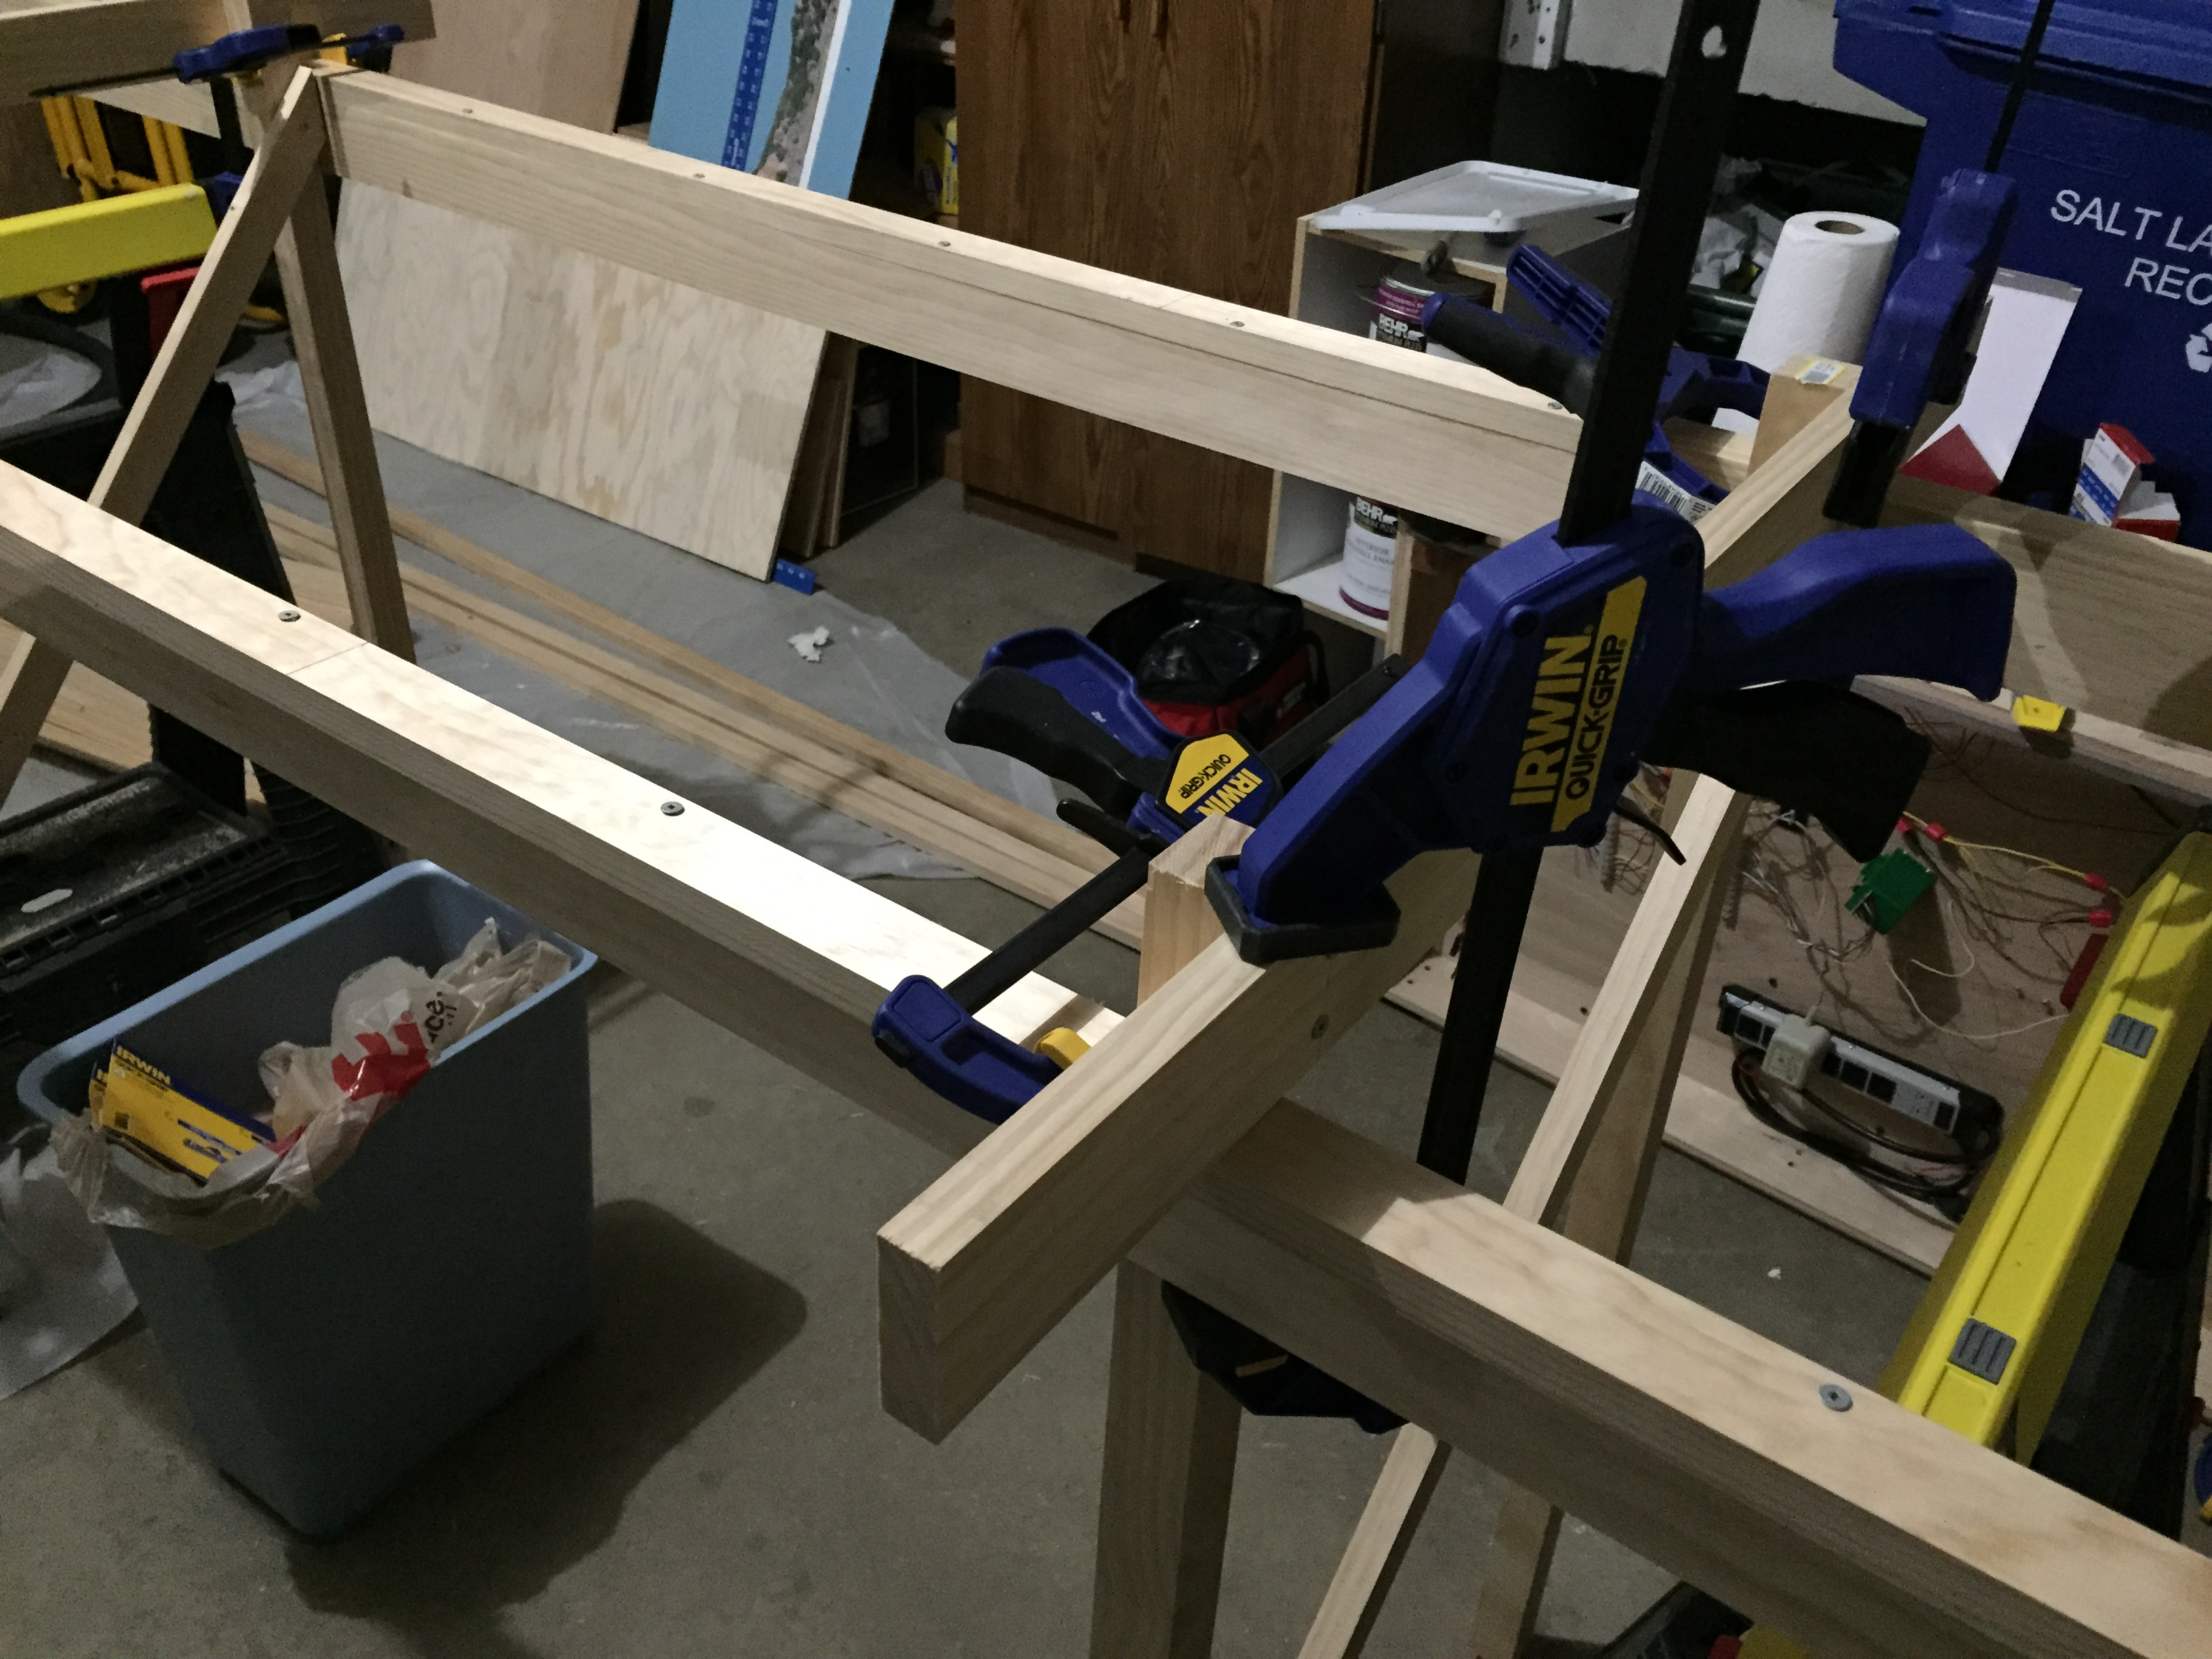
\includegraphics[width=0.5\textwidth]{title/figures/2014a.JPG}%
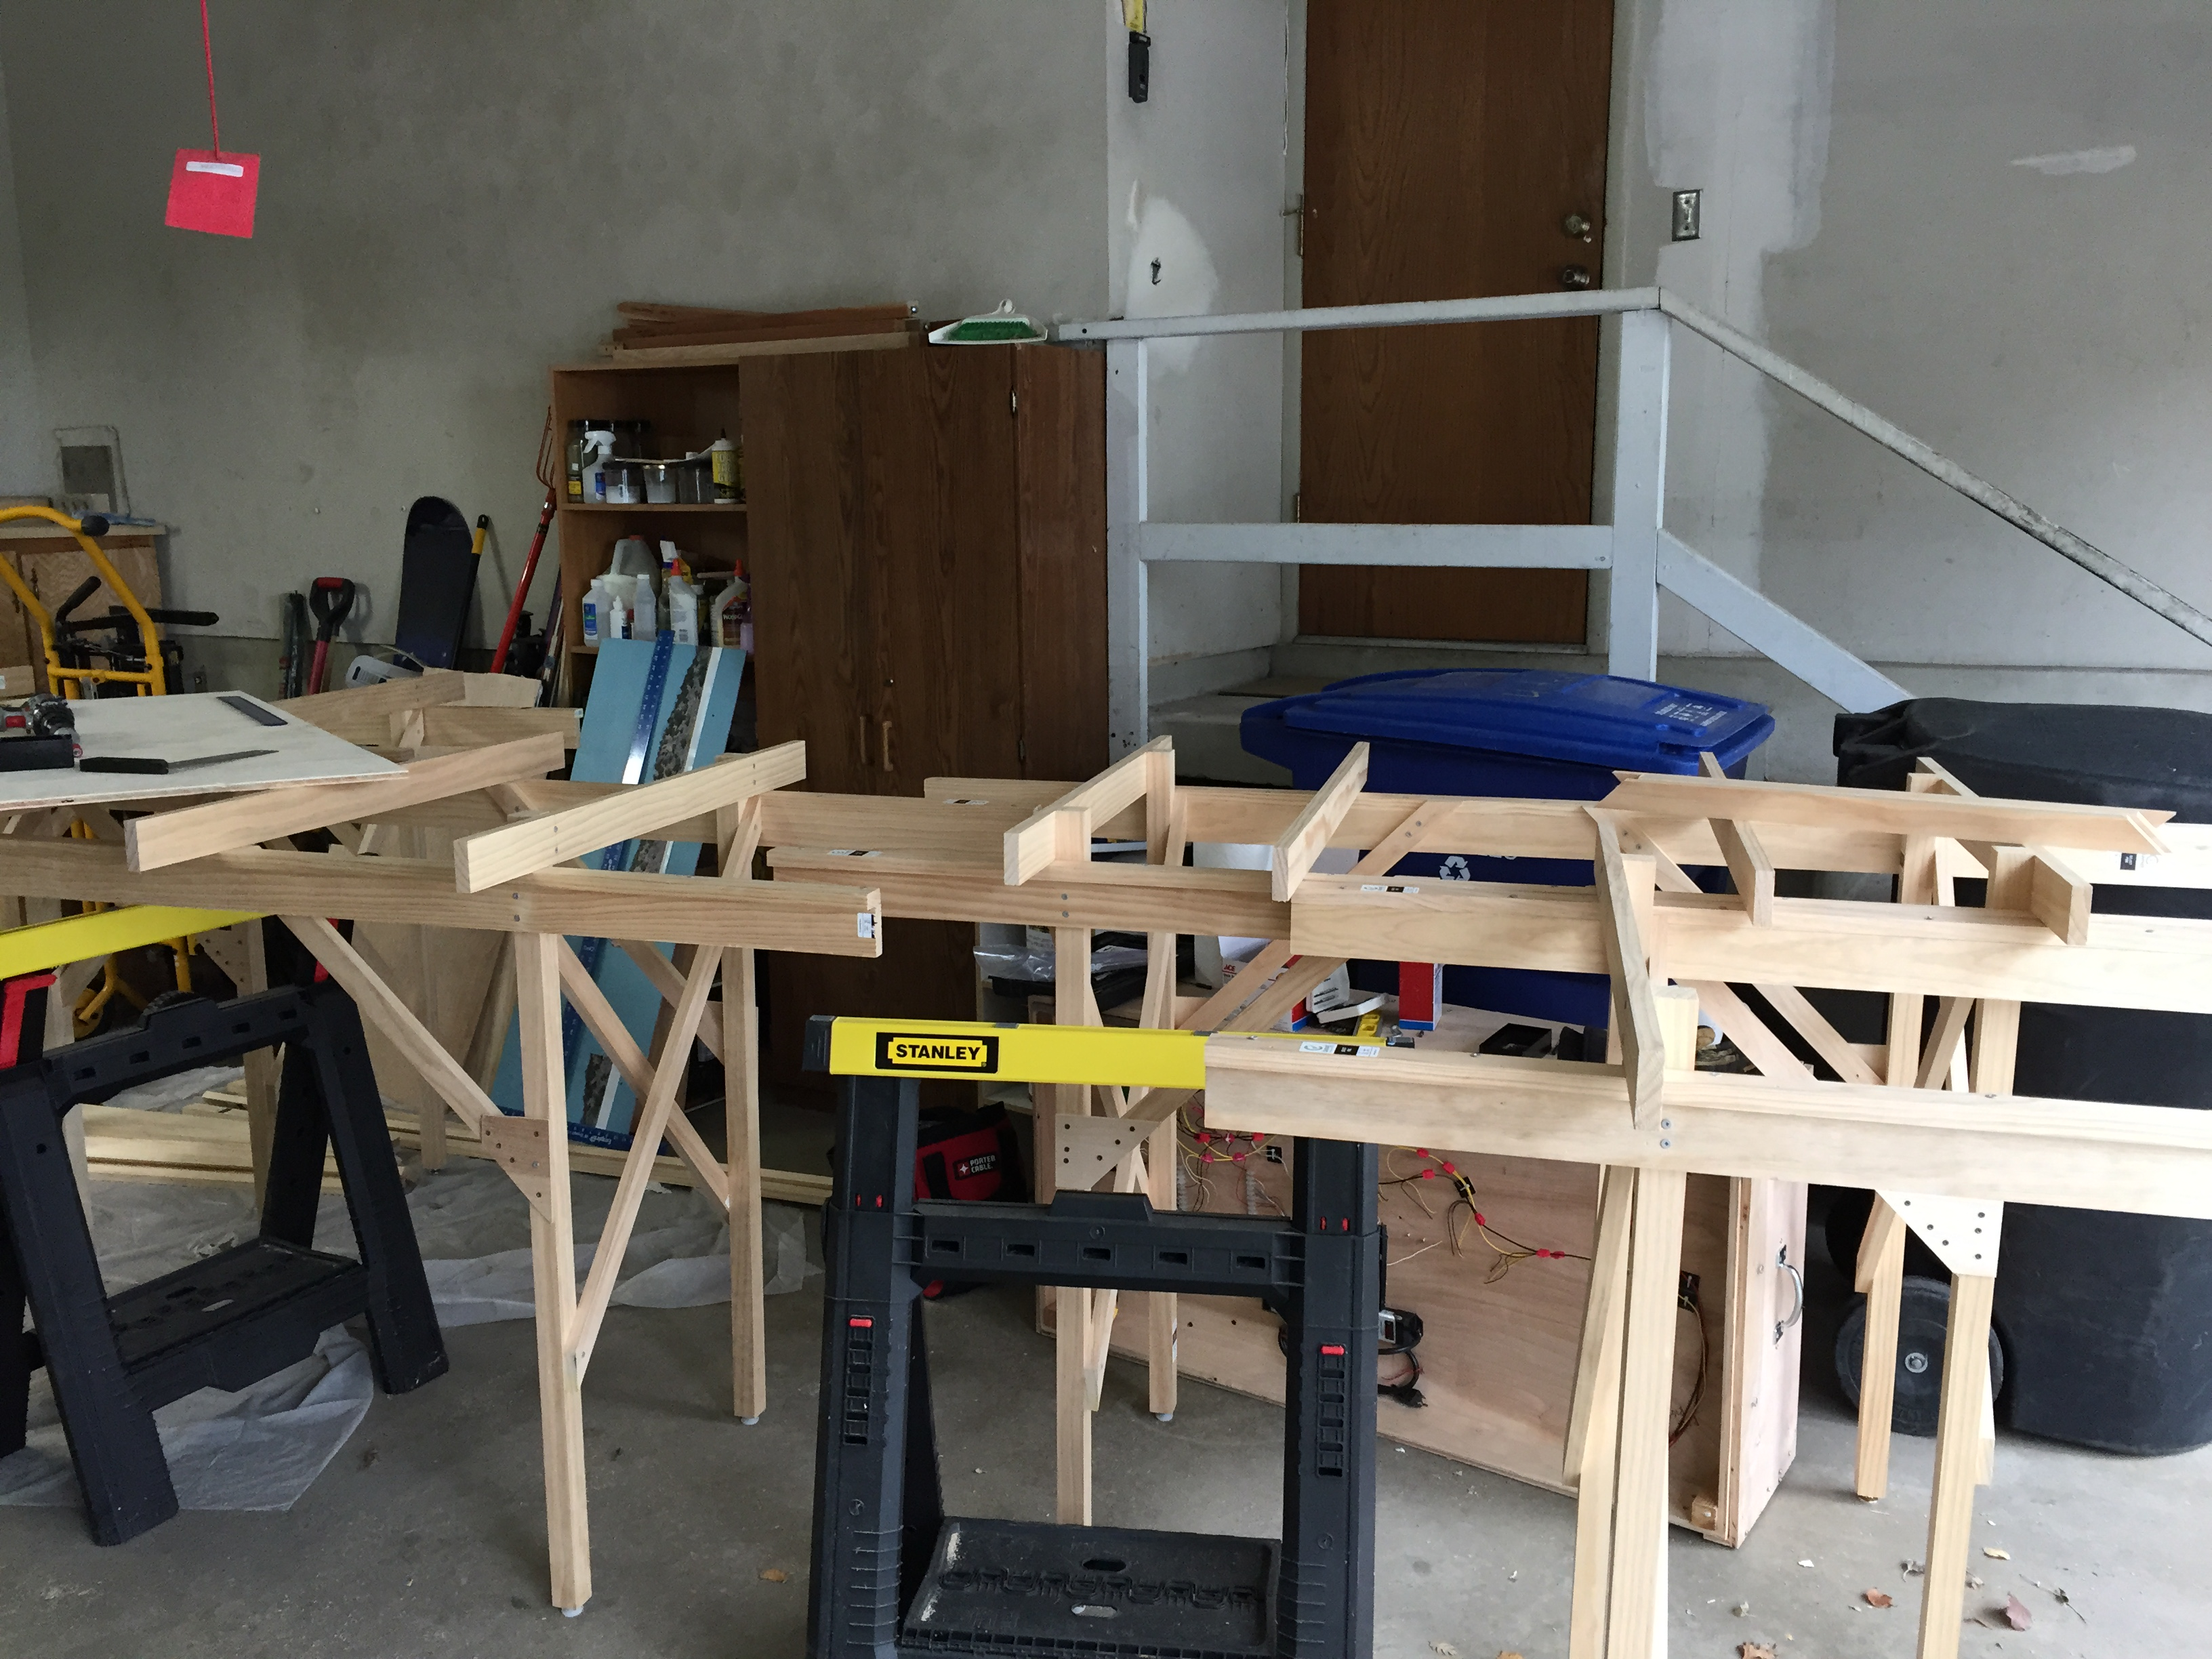
\includegraphics[width=0.5\textwidth]{title/figures/2014b.JPG}\par\nointerlineskip
\includegraphics[width=0.3333\textwidth,angle=180]{title/figures/2026a.jpeg}%
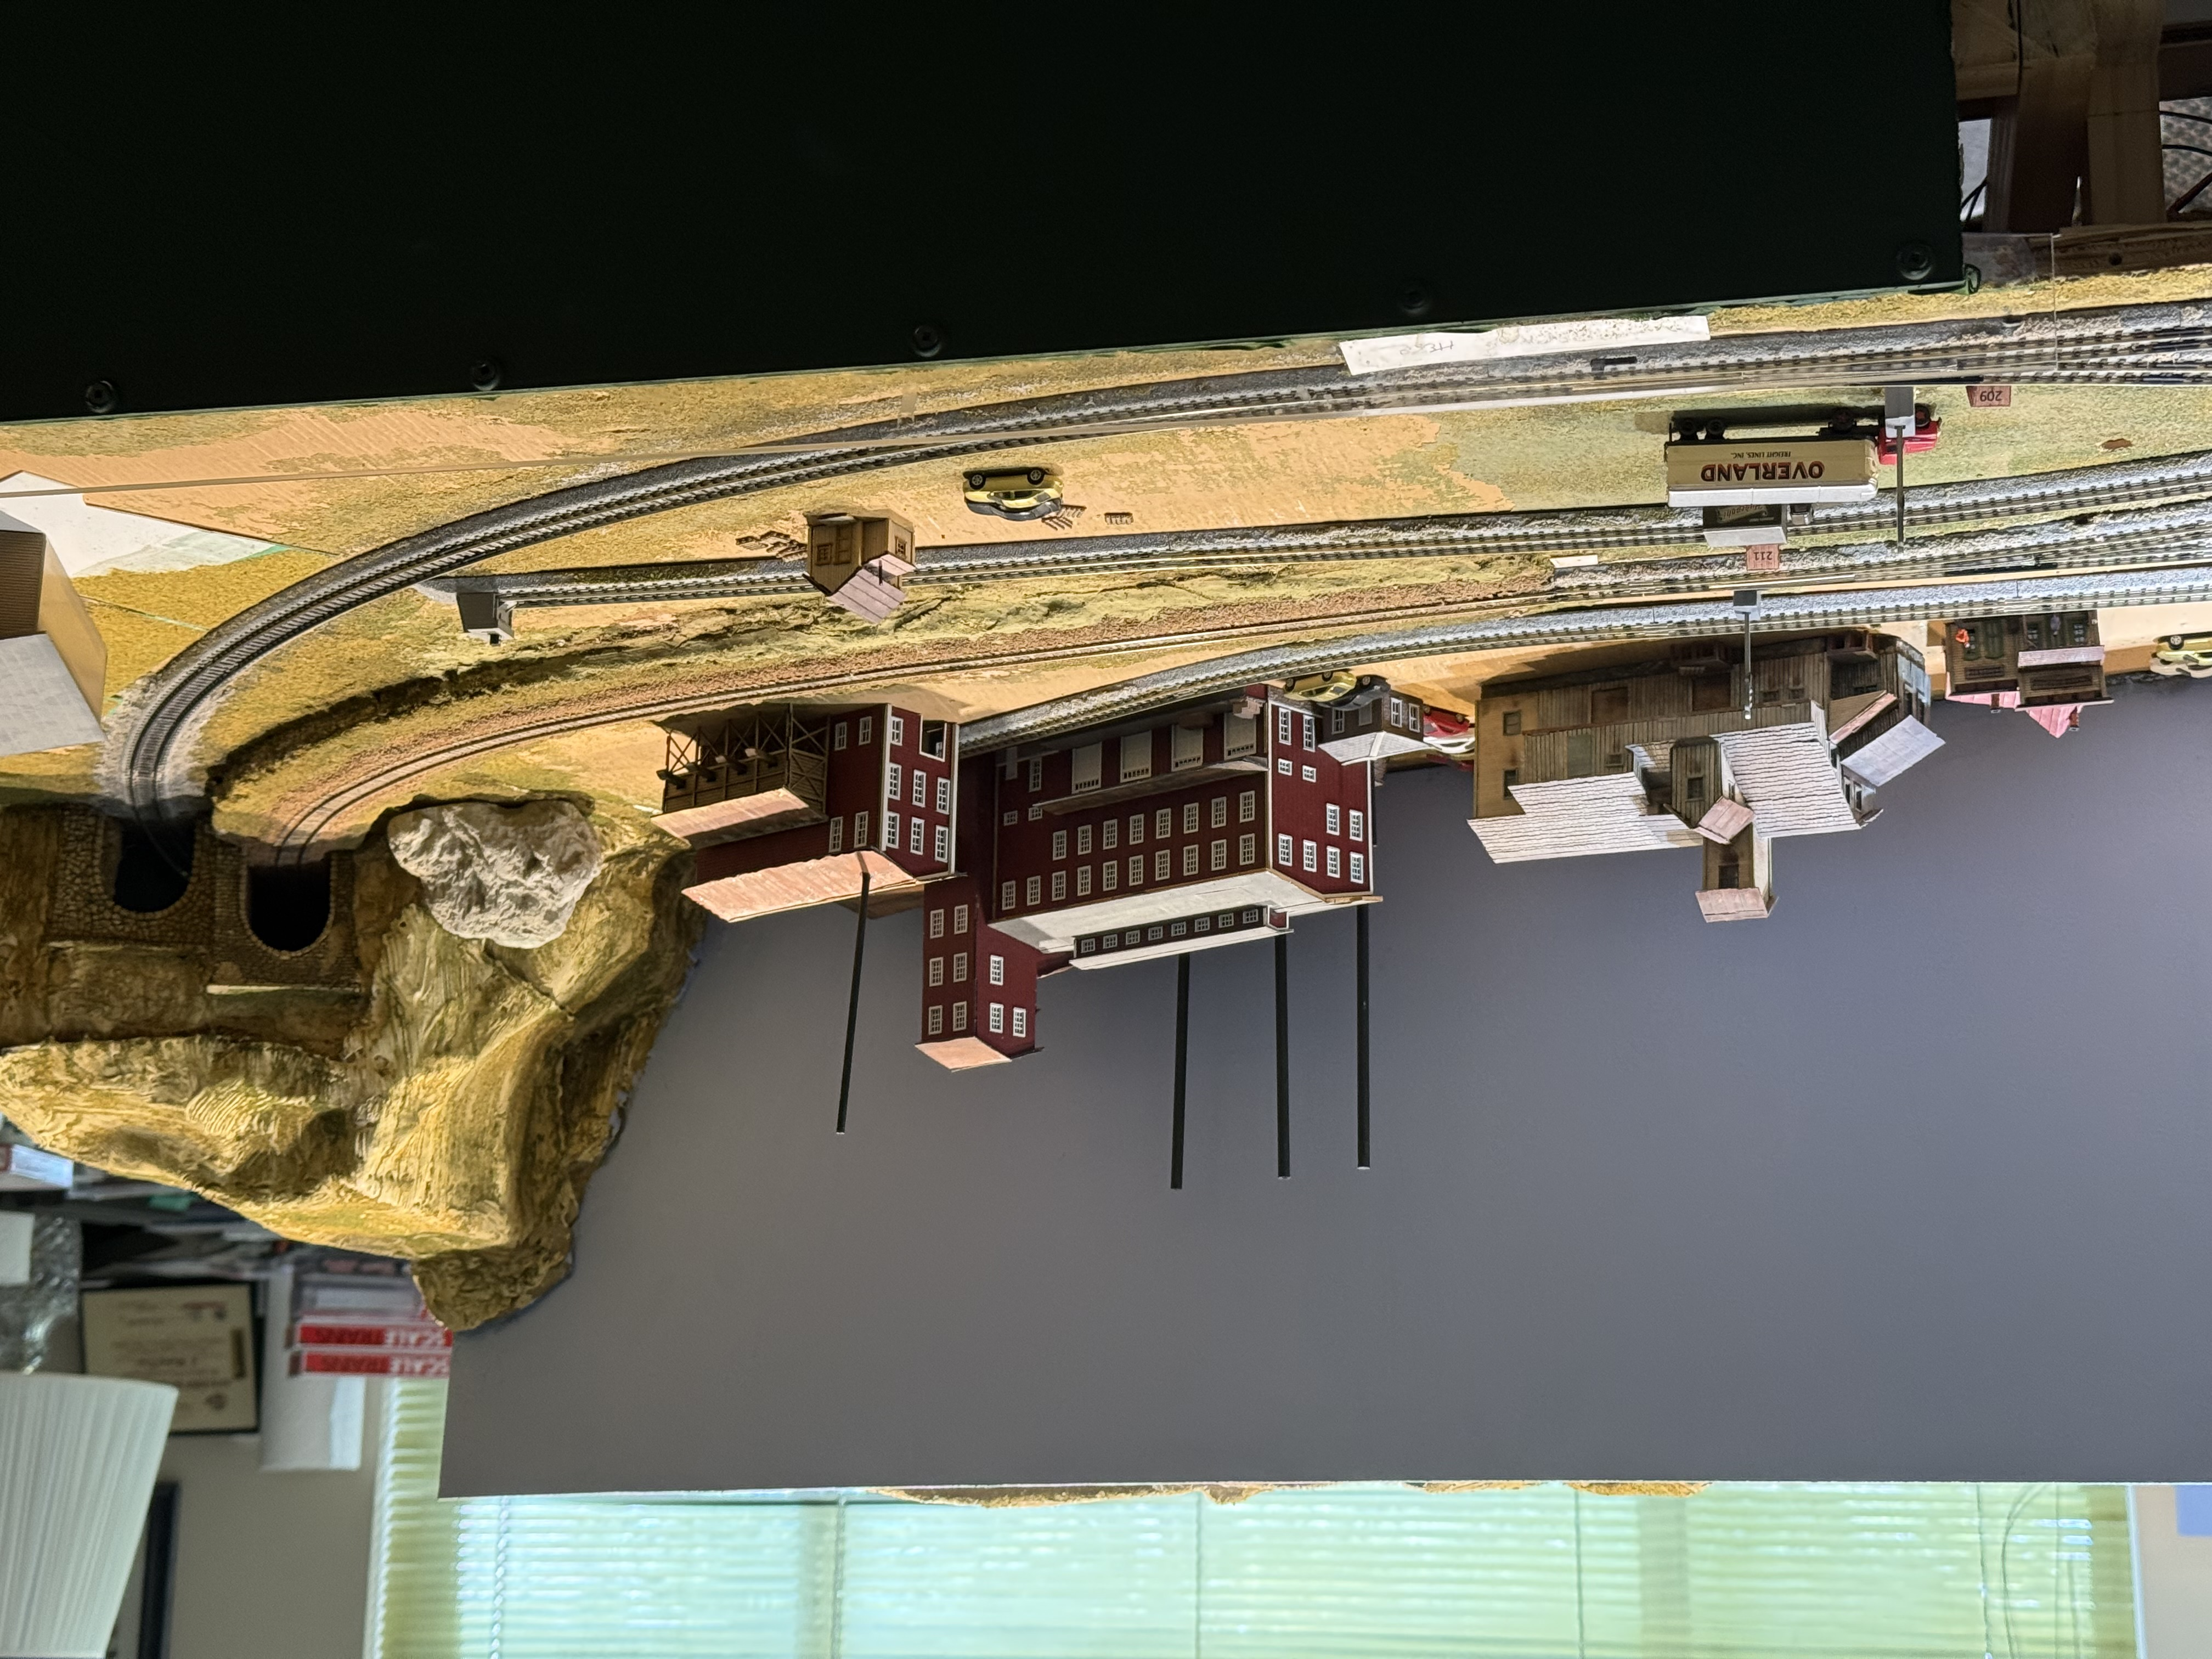
\includegraphics[width=0.3333\textwidth,angle=180]{title/figures/2026b.jpeg}%
\includegraphics[width=0.3334\textwidth,angle=180]{title/figures/2026c.jpeg}}%
\end{minipage}}

\vspace{\stretch{1}}

\noindent\hspace*{\centeroffset}\makebox[0pt][l]{\begin{minipage}{\textwidth}

\flushright

Printing Date: \today
\end{minipage}}
\vspace{\stretch{2}}


\endinput 

\dominitoc
\tableofcontents
\listoftables
\listoffigures
\chapter{Preface}

%%%% Main matter of the book
\mainmatter
\pagestyle{protocol}
\part{Wasatch N Scale Club}
\include{wasatch_n_scale/module}


\part{Basement Layout}
%\include{basement/basement}
%% This document describes Electrical AP Certificate for the railroad project.
%
%  				J. Michael Dean, M.D.
%  				University of Utah School of Medicine

% The following line makes this document point back so that my software will synchronize
% between the preview and source windows.

%!TEX root = ../Railroad.tex

\chapter{Electrical AP Certificate}
%\minitoc
%\index{test}

%\include{civil/civil}
%% This document describes Structures AP Certificate for the railroad project.
%
%  				J. Michael Dean, M.D.
%  				University of Utah School of Medicine

% The following line makes this document point back so that my software will synchronize
% between the preview and source windows.

%!TEX root = ../Railroad.tex

\chapter{Structures AP Certificate}
%\minitoc
%\index{test}

%\include{scenery/scenery}

\part{JMRI Configuration Using GIT}
%% This document describes Git version control for the railroad project.
%
%  				J. Michael Dean, M.D.
%  				University of Utah School of Medicine

% The following line makes this document point back so that my software will synchronize
% between the preview and source windows.

%!TEX root = ../Railroad.tex

\chapter{Git}
%\minitoc
%\index{test}

%% This document describes JMRI configuration for the railroad project.
%
%  				J. Michael Dean, M.D.
%  				University of Utah School of Medicine

% The following line makes this document point back so that my software will synchronize
% between the preview and source windows.

%!TEX root = ../Railroad.tex

\chapter{Java Model Railroad Interface}
\minitoc
%\index{test}
\section{Introduction}
The Java Model Railroad Interface (JMRI) is a Java program that has been under active development and support since October 1999;  the project
is an open source project that by October 2024 had had over 10,000 updates from over 300 developers world wide.  It's components include software 
for programming decoders, creating layouts, automating signaling, allowing automatic trains, and much much more.  I have been using JMRI for managing decoders,
setting up current based occupancy detection, train control over Wifi, scripted running of trains using Jython, automating turnouts and routes, and creating meaningful signaling animation.  It can also be used to create switch lists for operations, and many other aspects of model railroading.  The main website is \url{https://www.jmri.org} and relevant software resources are maintained on GitHub at \url{https://github.com/JMRI}.

This chapter is not intended as a tutorial or reference manual for JMRI.  It is a description of how I have configured JMRI for my own use.

\section{Architecture Summary}
The program has been designed to be easy for model railroaders to configure, relying heavily on the use of tables.  These tables contain objects such as 
sensor, turnouts, lights, signal masts, etc. and users can configure the system directly with these tables.  When the computer is hooked up to the layout via a DCC system or other connection, manipulation of table values will physically affect the layout.  Thus, in the turnout table, if the user clicks on the button to throw the turnout, it will actually happen on the layout.  All the settings of JMRI are contained in an XML file that includes all parameters in the system as well as details
about the layout.  It is also possible to save individual XML files for specific items such as turnouts, and this has been a historical source of user confusion.
For our purposes, ALL settings are saved in a single XML file for each railroad layout.

Why would we have more than one layout in JMRI?  An easy example is having a programming track;  if DecoderPro is used to manage the decoders of
locomotives and this is accomplished on a programming track, we would like to save the roster settings somewhere where PanelPro can access the information when it is running the main layout.  In my case, I have four different JMRI layout configurations:
\begin{compactitem}
	\item{Basement Revised 2024}
	\item{Decoder\_TestTrack}
	\item{My\_NCE\_Simulator}
	\item{Programming\_Track}
\end{compactitem}

My main layout is in the basement, and my programming track is attached to that layout.  The Decoder test track is a separate module that I constructed for
automated speed matching of locomotives, and the NCE simulator is a completely fake layout that I can use to explore features of JMRI without a physical
equivalent.

After installation, the user can configure where the files are for his or her specific situation, and then when JMRI is updated, no changes have to be made.
I have a JMRI folder in my home directory, and it's structure is shown in Figure \vref{fig:jmri-file-structure}.

\begin{figure}[htbp]
\begin{filetree}
JMRI/
+-- Basement_Revised_2024.jmri/     Main layout profile
|   +-- profile/
|   |   +-- profile.xml             Connection config and startup actions
|   |   +-- profile.properties      Preferences: roster path, web server
|   |   +-- 5e82e5b0-.../           Machine-specific profile overrides
|   |   |   +-- profile.xml
|   |   |   +-- profile.properties
|   |   |   +-- user-interface.xml
|   |   +-- d2a3bcad-.../           Machine-specific profile overrides
|   |       +-- profile.xml
|   |       +-- profile.properties
|   |       +-- user-interface.xml
|   +-- March2026Settings.xml       Current panel/layout configuration
|   +-- May2025Settings.xml         Previous panel versions
|   +-- April2025Settings.xml
|   +-- October2022Settings.xml
|   +-- backupPanels/               Timestamped automatic backups
|   +-- signal/
|   |   +-- WarrantPreferences.xml
|   +-- throttle/
|   |   +-- ThrottlesPreferences.xml
|   |   +-- WiThrottlePreferences.xml
|   +-- programmers/                Custom decoder programmer configs
|   +-- resources/                  Custom icons, images
|   +-- roster.xml                  Profile-local roster reference
+-- Decoder_TestTrack.jmri/         Decoder calibration testing profile
+-- My_NCE_Simulator.jmri/         Simulation without hardware
+-- Programming_Track.jmri/         Programming track profile
+-- roster/                         Shared locomotive roster
+-- jython/                         Shared Jython scripts
+-- roster.xml                      Master roster index
+-- roster.csv                      CSV export of roster
\end{filetree}
\caption{JMRI directory structure}
\label{fig:jmri-file-structure}
\end{figure}

Each \texttt{.jmri} profile directory follows the same structure shown above for \texttt{Basement\_Revised\_2024.jmri}.  The machine-specific UUID subdirectories under \texttt{profile/} allow different machines to have their own UI and connection preferences while sharing the same layout configuration.

\section{Roster}
The \texttt{roster/} directory is shared across all profiles.  Each profile points to it via \texttt{jmri-jmrit-roster.directory=home:JMRI/} in its \texttt{profile.properties}, so there is only one copy of each locomotive definition regardless of which profile is active.  The root-level \texttt{roster.xml} is the master index that JMRI uses to find individual locomotive files.

Each locomotive has an XML file containing its DCC address, decoder CV settings, function labels, and other configuration.  Many also have a corresponding photo. (See Figure \vref{fig:roster-structure}.

\begin{figure}[htbp]
\begin{filetree}
roster/
+-- consist/
|   +-- consist.xml                 Consist definitions
+-- Big_Boy_4_8_8_4.xml             Locomotive definition - DCC/CV config
+-- BigBoySide.jpeg                 Corresponding photo
+-- 1029_NW2_Switcher.xml
+-- up1029.jpg
+-- ... (45+ locomotive XML files and 20+ photos)
\end{filetree}
\caption{Roster directory structure}
\label{fig:roster-structure}
\end{figure}

\part{3D Printing}
% This document describes 3D printing setup for reference.
%
%  				J. Michael Dean, M.D.
%  				University of Utah School of Medicine

% The following line makes this document point back so that my software will synchronize
% between the preview and source windows.

%!TEX root = ../Railroad.tex

\chapter{3D Printing for Railroad}
\minitoc

\section{Ender 3 Printer from Creality}

I have mostly ignored 3d printing because of the high cost of these printers.  In December 2018, about two weeks before Christmas with all kinds of family in the house,
I ordered the Ender 3 printer from Creality.  This printer had (and still has) established notoriety because of its relatively high quality print
capability and a cost that was sometimes under \$200.  The printer comes as a kit that has to be assembled, but the major complex pieces are already
assembled.  I found an incredibly helpful video on YouTube that helped understand the instructions.  The major issue is assuring that the frame is put together square.\\

After assembly, I ran a test print from the included SD card, ending up with a dog.  After this, of course, one has to find things to print or figure out how to design
items on the computer using various pieces of software.  ThingiVerse is a web site with thousands of files that can be downloaded and printed, but certain things
simply cannot be printed with a fused deposition modeling (FDM) type of printer.  The Ender 3 is an FDM printer.  This heats up plastic and deposits it in layers, and after depositing one layer, the print head rises 0.1 to 0.2 mm (depending on settings) and deposits the next layer.  Extremely small or detailed parts do not print well,
and it is possible to end up with a mess of plastic spaghetti with certain patterns.  If I want to get into small detailed parts, I will be forced to buy a different type of 3d printer based on stereolithography (resin printers).  At the time of this writing, in December 2019, I will defer on this next technology.

\section{Original Prusa i3 MK3S Printer}
In July 2020, in the midst of my fifth month in pandemic experience, I ordered the Prusa printer in kit form, which arrived in August.  The kit was challenging to build, but now I understand how the printer works.  I was reasonably careful, and the machine has worked very well.  Its primary advantages include filament detection, autoloading, autounloading, automatic bed leveling, and Z-level adjustments.  It is also a direct extrusion machine (not a Bowden tube machine) and has a far superior extrusion mechanism compared with the Ender.

\section{Setting up Octoprint with Raspberry Pi}

I decided to try a piece of software called Octoprint.  The first step was to 3d print some parts that will hold a camera for the Raspberry PI, as well as some enhancements
of the Ender 3.  This was bizarre (enhancing my printer by printing enhancement parts).  After I replaced the Ender 3 with my Prusa machine, I had to print a different set of parts, which was easily accomplished.  The camera enables me to see the status of the print, and also allows creating a time lapse movie of the overall print.\\

The settings are to make sure my desktop computer is on the DeanEERO, because the Pi is on DeanEERO.  Then I simply go to a browser
and aim at http://octopi.local and it logs into the Raspberry Pi with the interface for controlling the printer.  I don't have to mess with the operating system or finding the software,
as this is automatically set up.  I need to upload files to the Pi in order for them to get printed, or alternatively, I can print from the SD
card that is in the printer.  I have noticed that if I print from the SD card, Octoprint does not have access to the GCODE, time lapse does not work, and it is possible to accidentally abort the print.  Therefore, I generally start an SD card print from the printer LCD and do not make any adjustments via the OctoPrint interface.\\


The user name is mdean77 and the password is Usual98a.  \\

\section{Development Process for 3d Parts}

There are several types of software available for doing 3D design on the computer.  Some are free, some are not.  I quickly became aware of Fusion 360, which is a high
end product that turns out to be completely free for hobbyists.  It has a steep learning curve, which I have attempted to climb, and it is certainly not the easiest option
available.  There are other products but Fusion is where I landed.  After completing a design, I export the file as an STL file.\\

The STL file now needs to be ``sliced'' into the individual layers that the FDM printer will lay down, one by one. The slicer software produces GCODE, which provides the printer with exact instructions for conducting the print.  I have three slicer software packages.  Cura was the first I used because it was included with the Ender 3, was free, and is very functional.  I purchased Simplify3D after a year, and this software allows having multiple processes.  This means that I can change settings in the middle of a print.  Finally, I have been using PrusaSlicer, which is provided in conjunction with the Original Prusa i3 MK3S printer that has replaced my Ender 3.  Each of these slicers has advantages and disadvantages, and it is unclear that any one of them is particularly superior to the others.\\

\section{Using Parts to Hide Accessory Decoders}
To learn Fusion 360 I found a tutorial that built a box with a snap on lid.  This led me to the idea of creating small boxes that could
contain the accessory decoders used to control my turnouts (Figure \ref{fig:naked}).  I have a large number of turnouts and it is obviously not an attractive seen to have decoders attached in haphazard manner.  For this reason, I created a box design that would contain the decoder and simplify the overall appearance (Figure \ref{fig:decoderInBox}).  Finally, I could make different versions depending on how many decoders were located in different areas of the layout, as shown in Figure \ref{fig:decoderBoxes}.

	\begin{figure}[htbp]
	\centering
	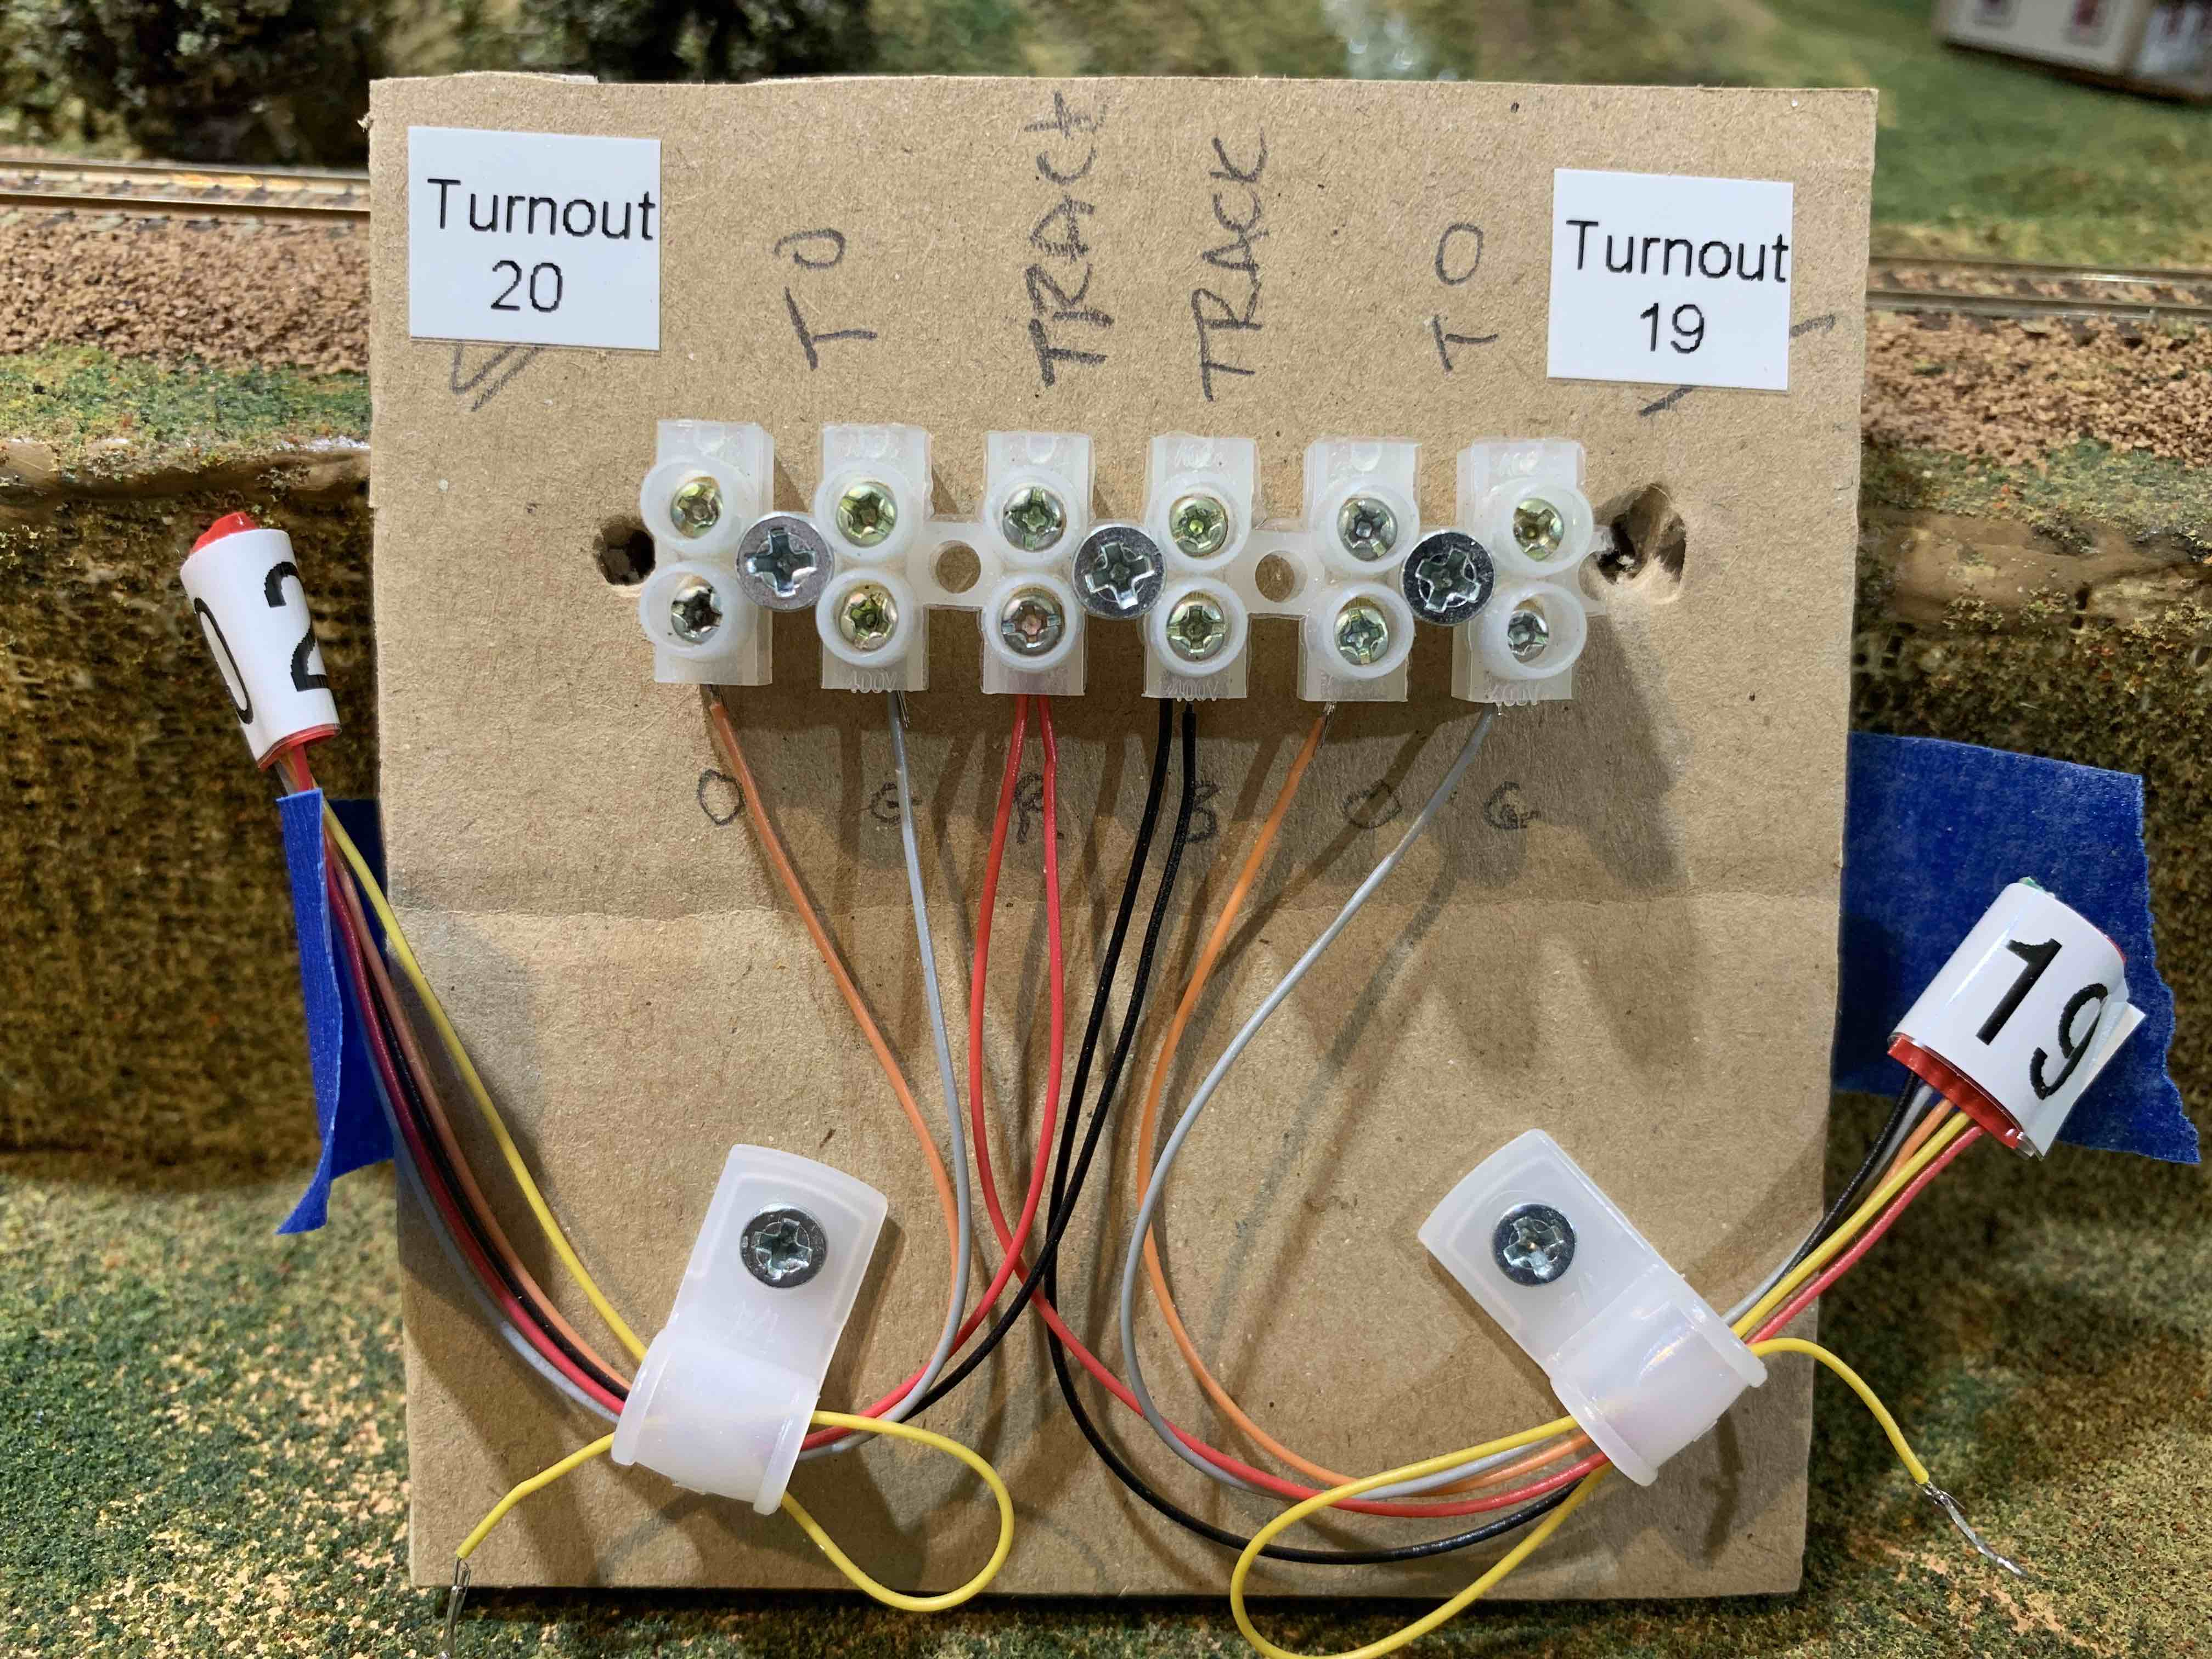
\includegraphics[width=0.4\textwidth]{./3d_printing/figures/TwoNakedDecoders.jpg}
	\caption{Accessory decoders taped to underside of layout.}
	\label{fig:naked}
	\end{figure}
	
	\begin{figure}[htbp]
	\centering
	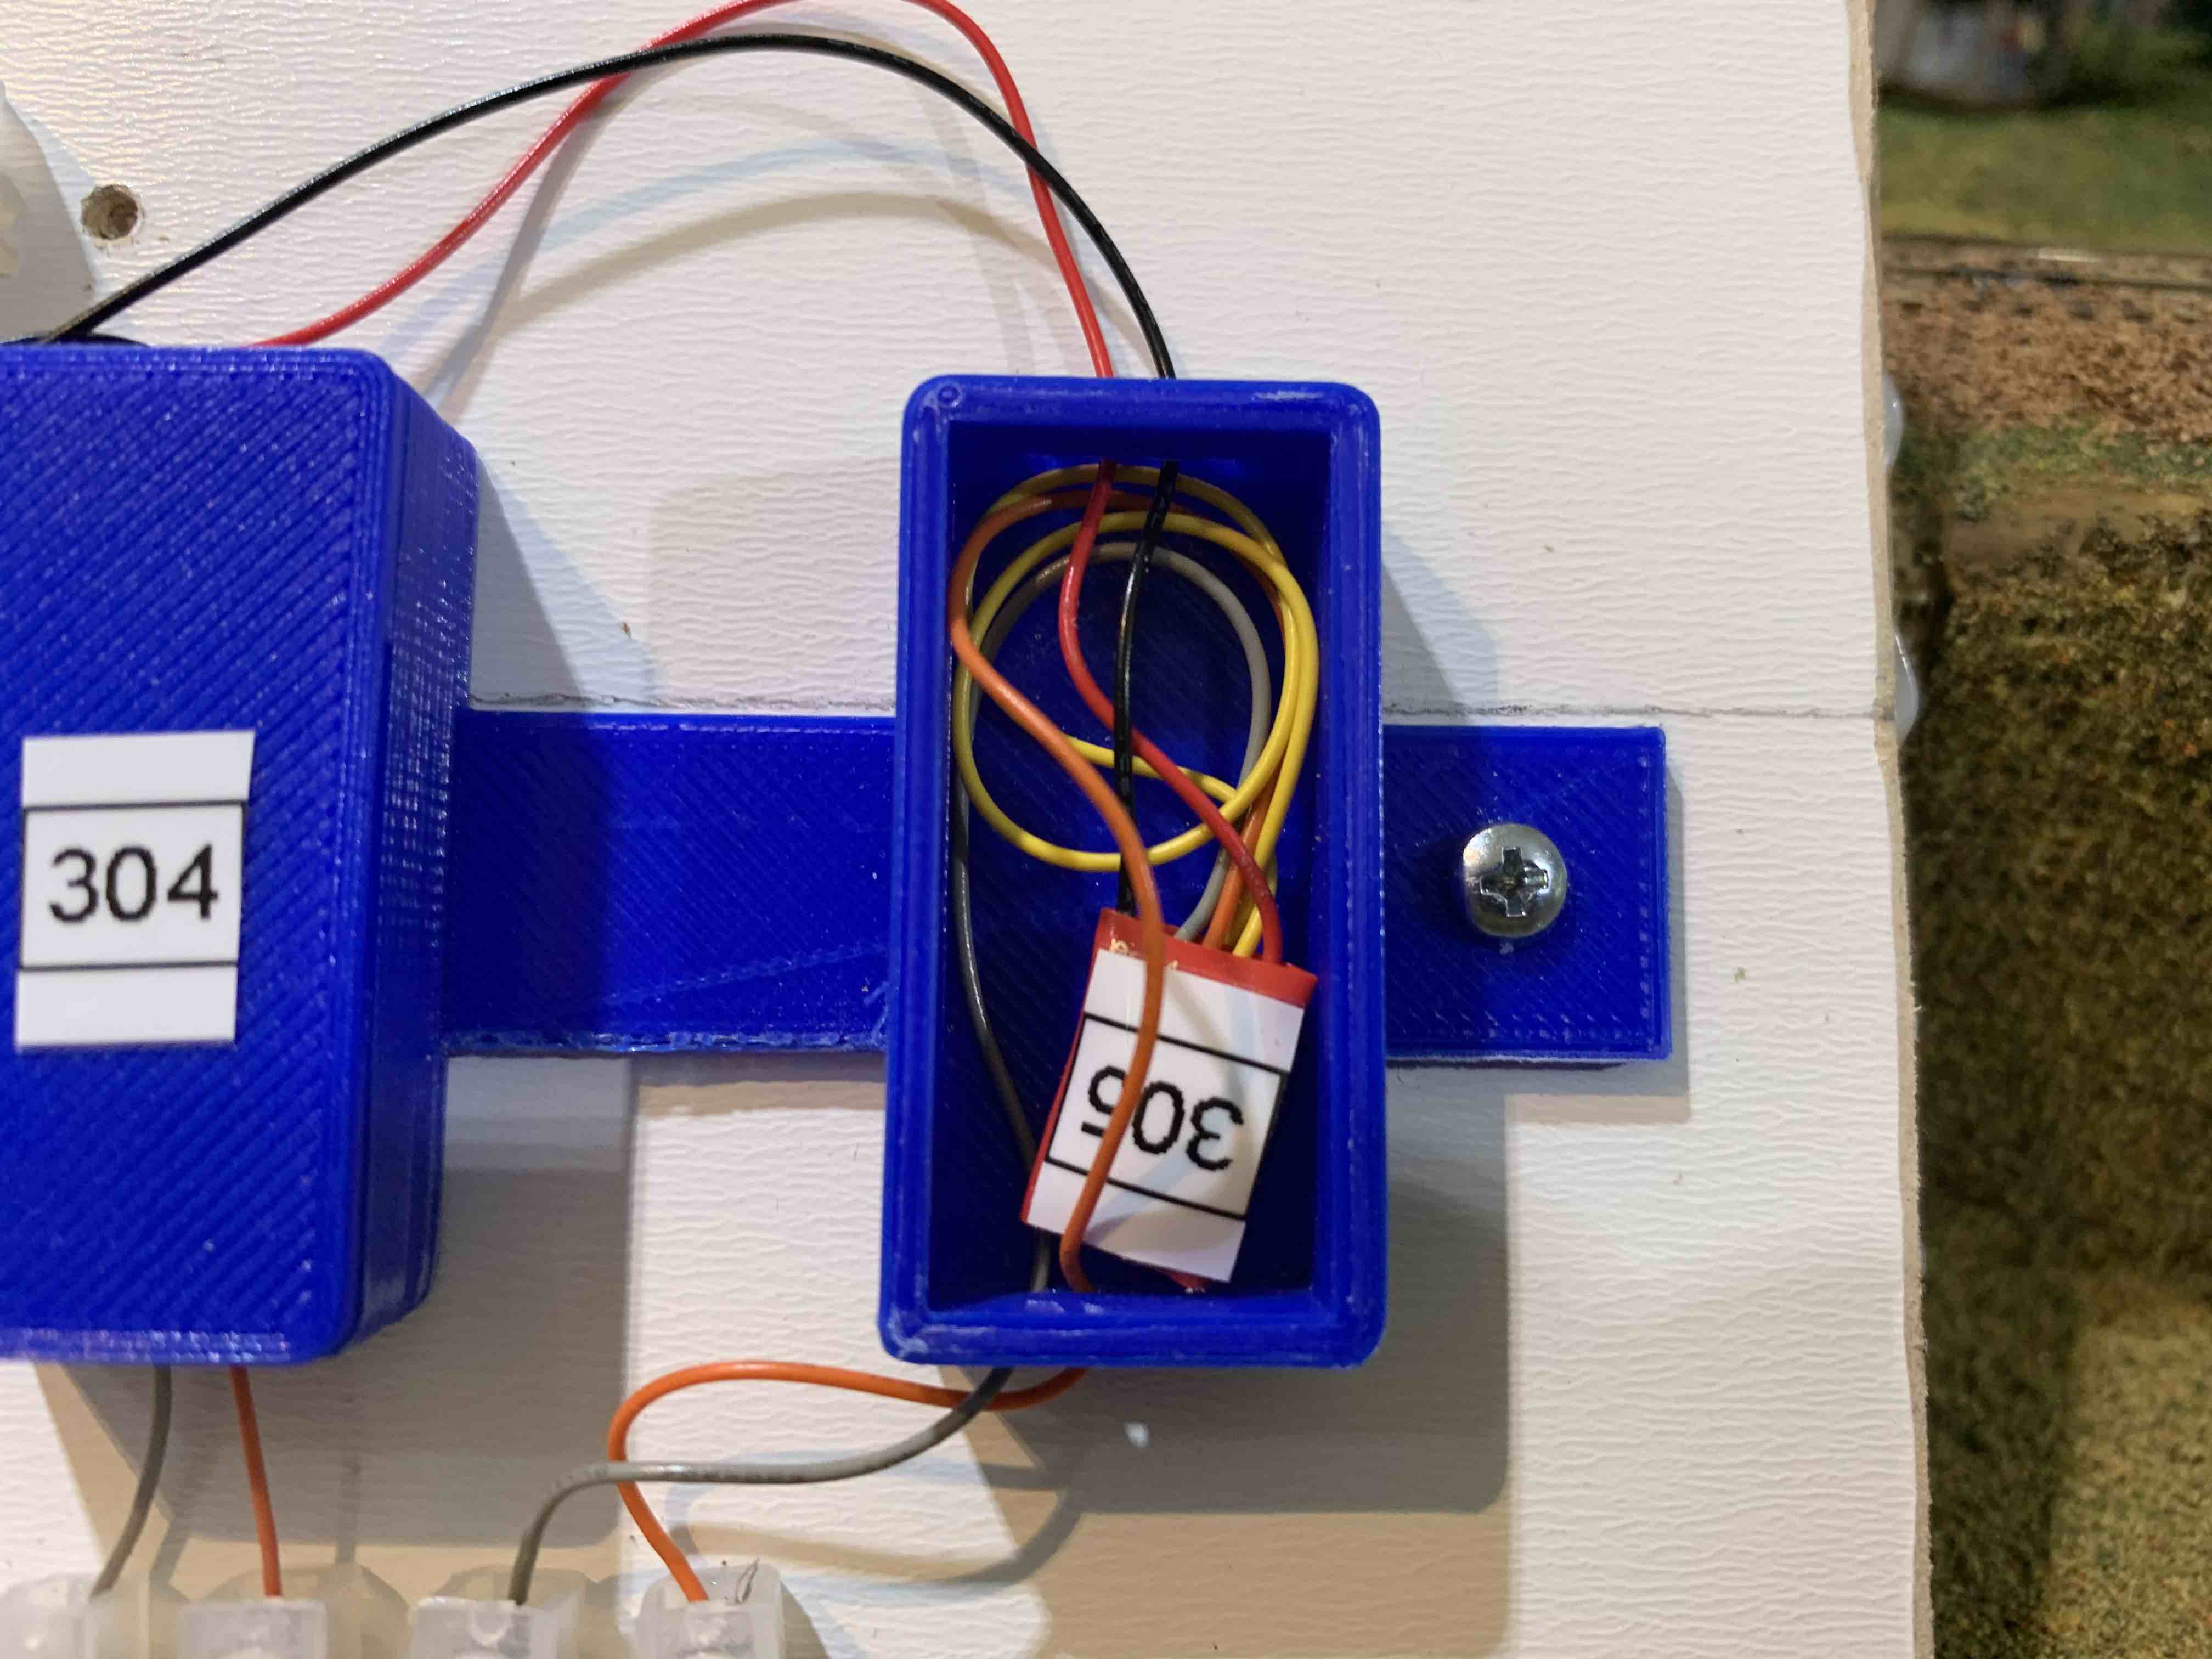
\includegraphics[width=0.4\textwidth]{./3d_printing/figures/DecoderInBox.jpg}
	\caption{Decoder in 3D box, simplifying the appearance.}
		\label{fig:decoderInBox}
	\end{figure}
	
    \begin{figure}[htpb]
        \centering
        \begin{subfigure}[b]{0.475\textwidth}
            \centering
            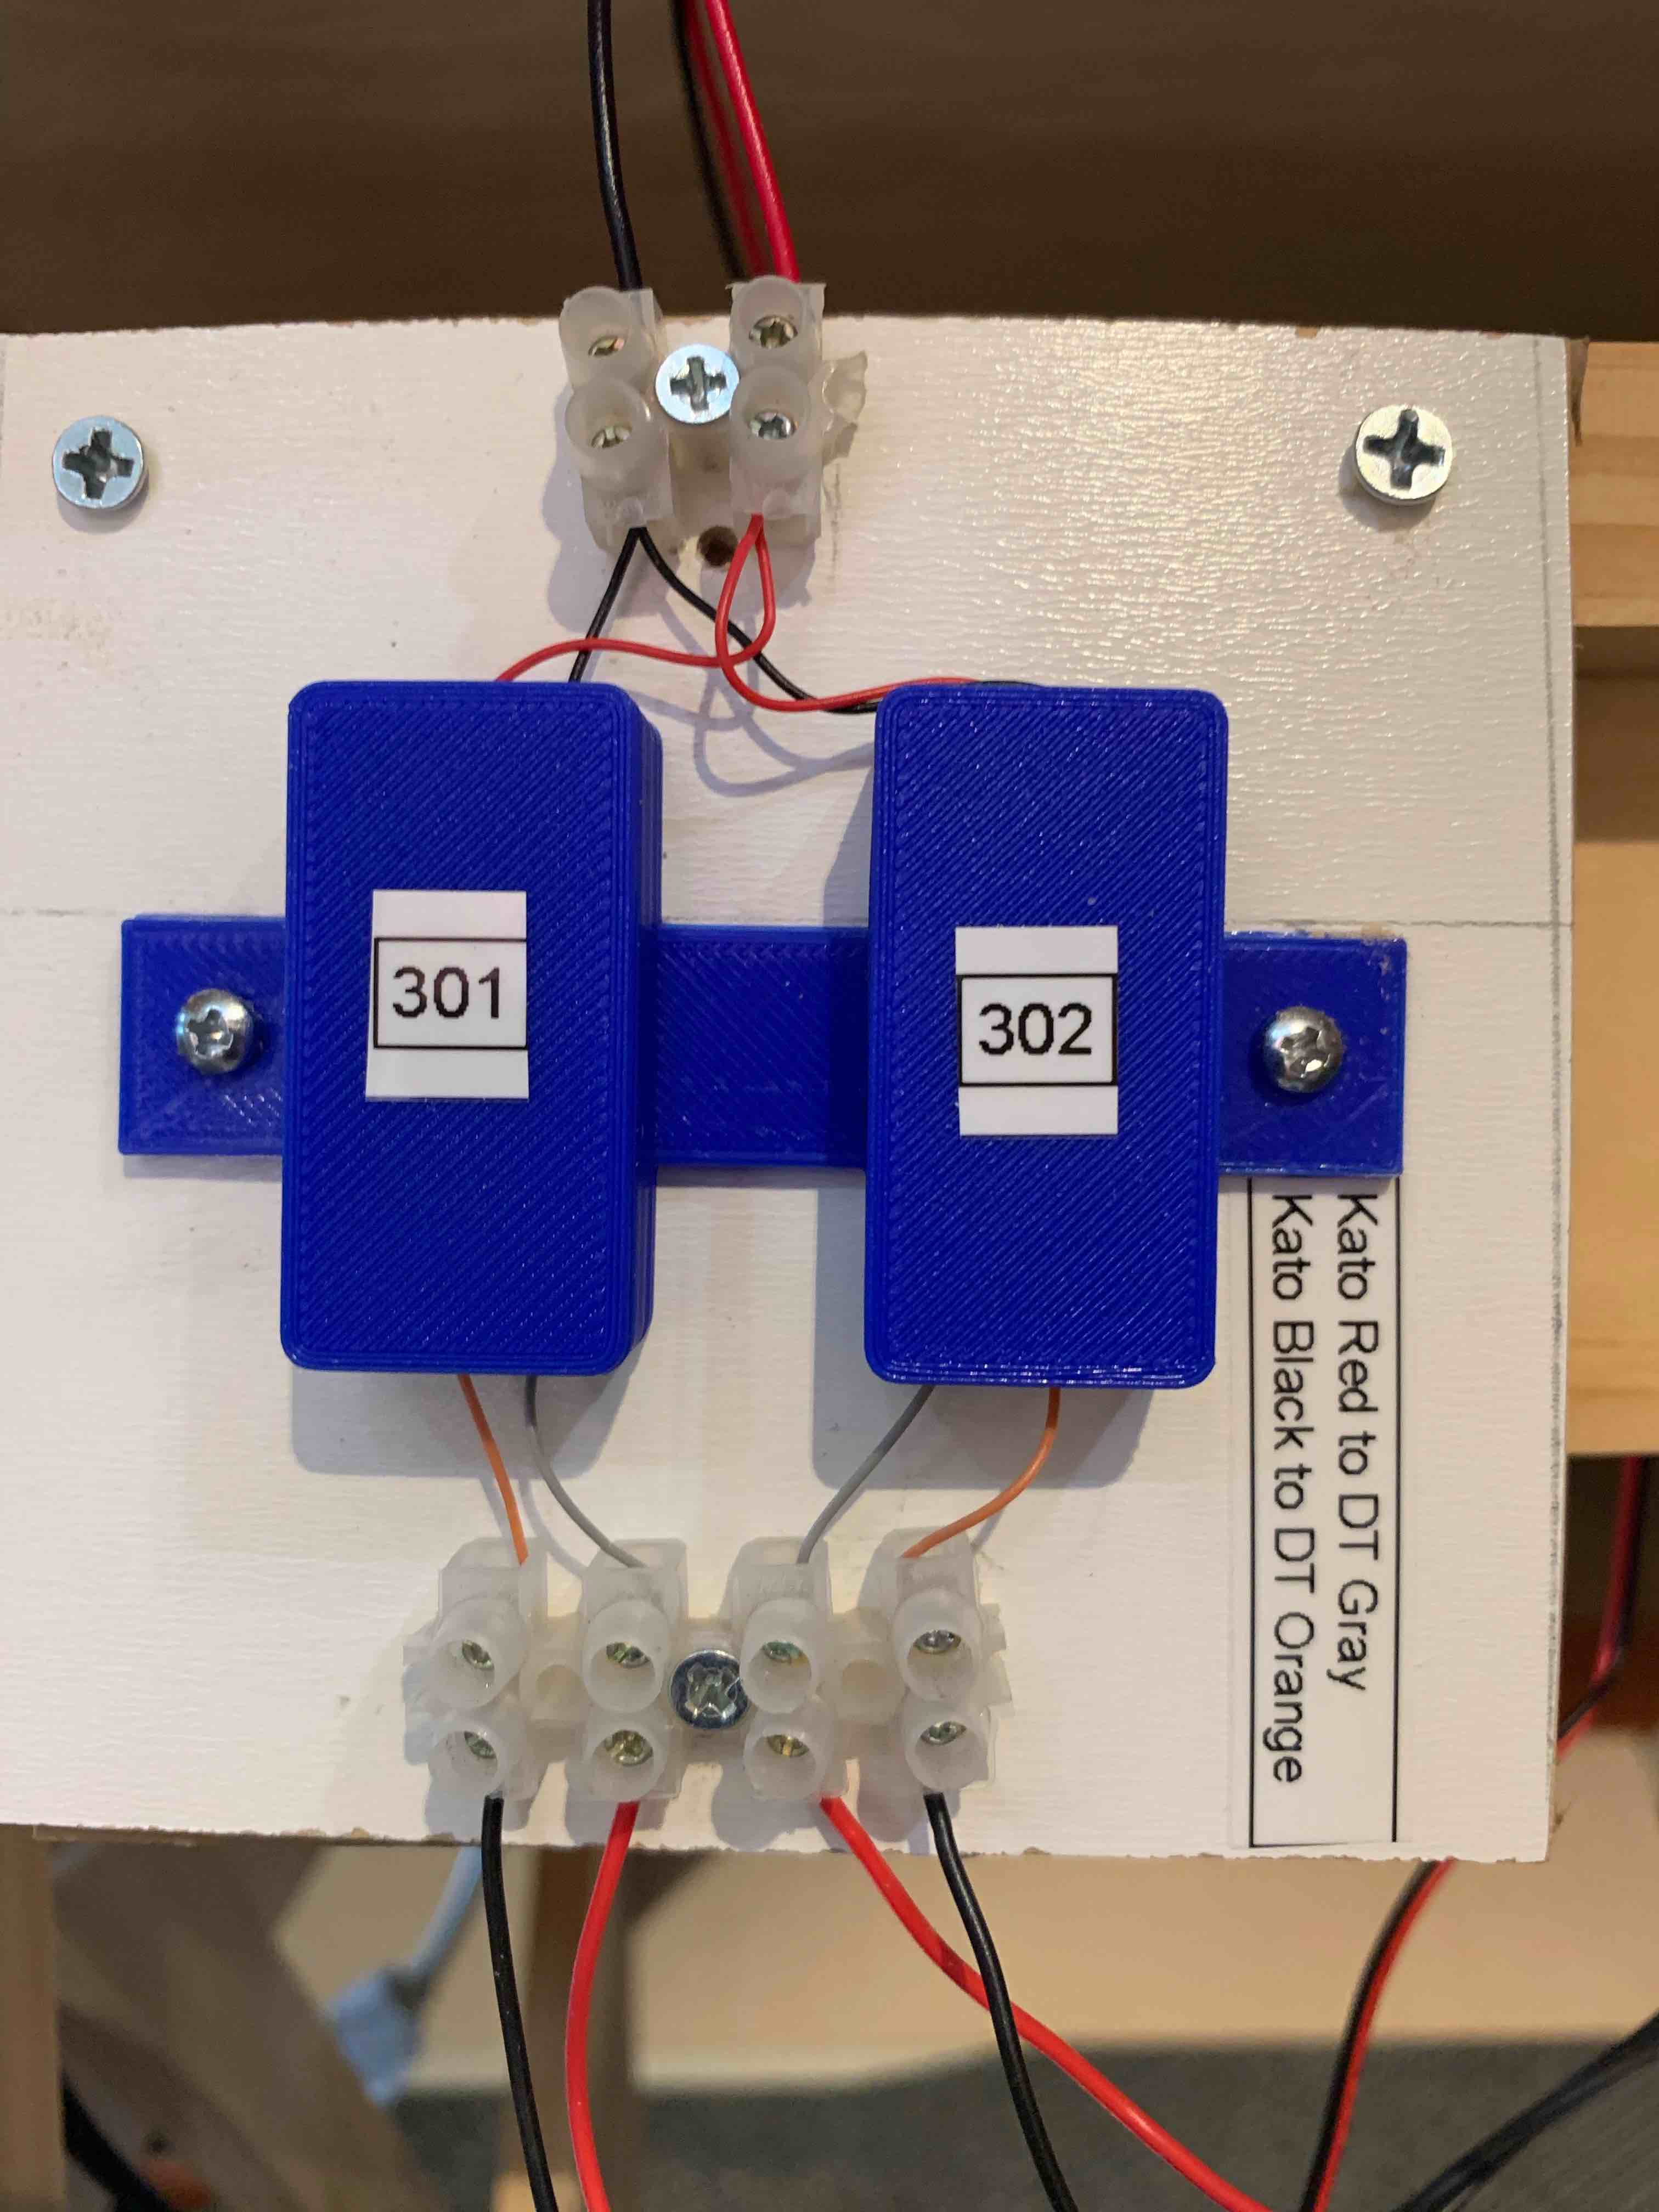
\includegraphics[width=\textwidth]{./3d_printing/figures/TwoBoxes.jpg}
           \caption{Print of two boxes}
        \end{subfigure}
        \hfill
        \begin{subfigure}[b]{0.475\textwidth}
            \centering 
            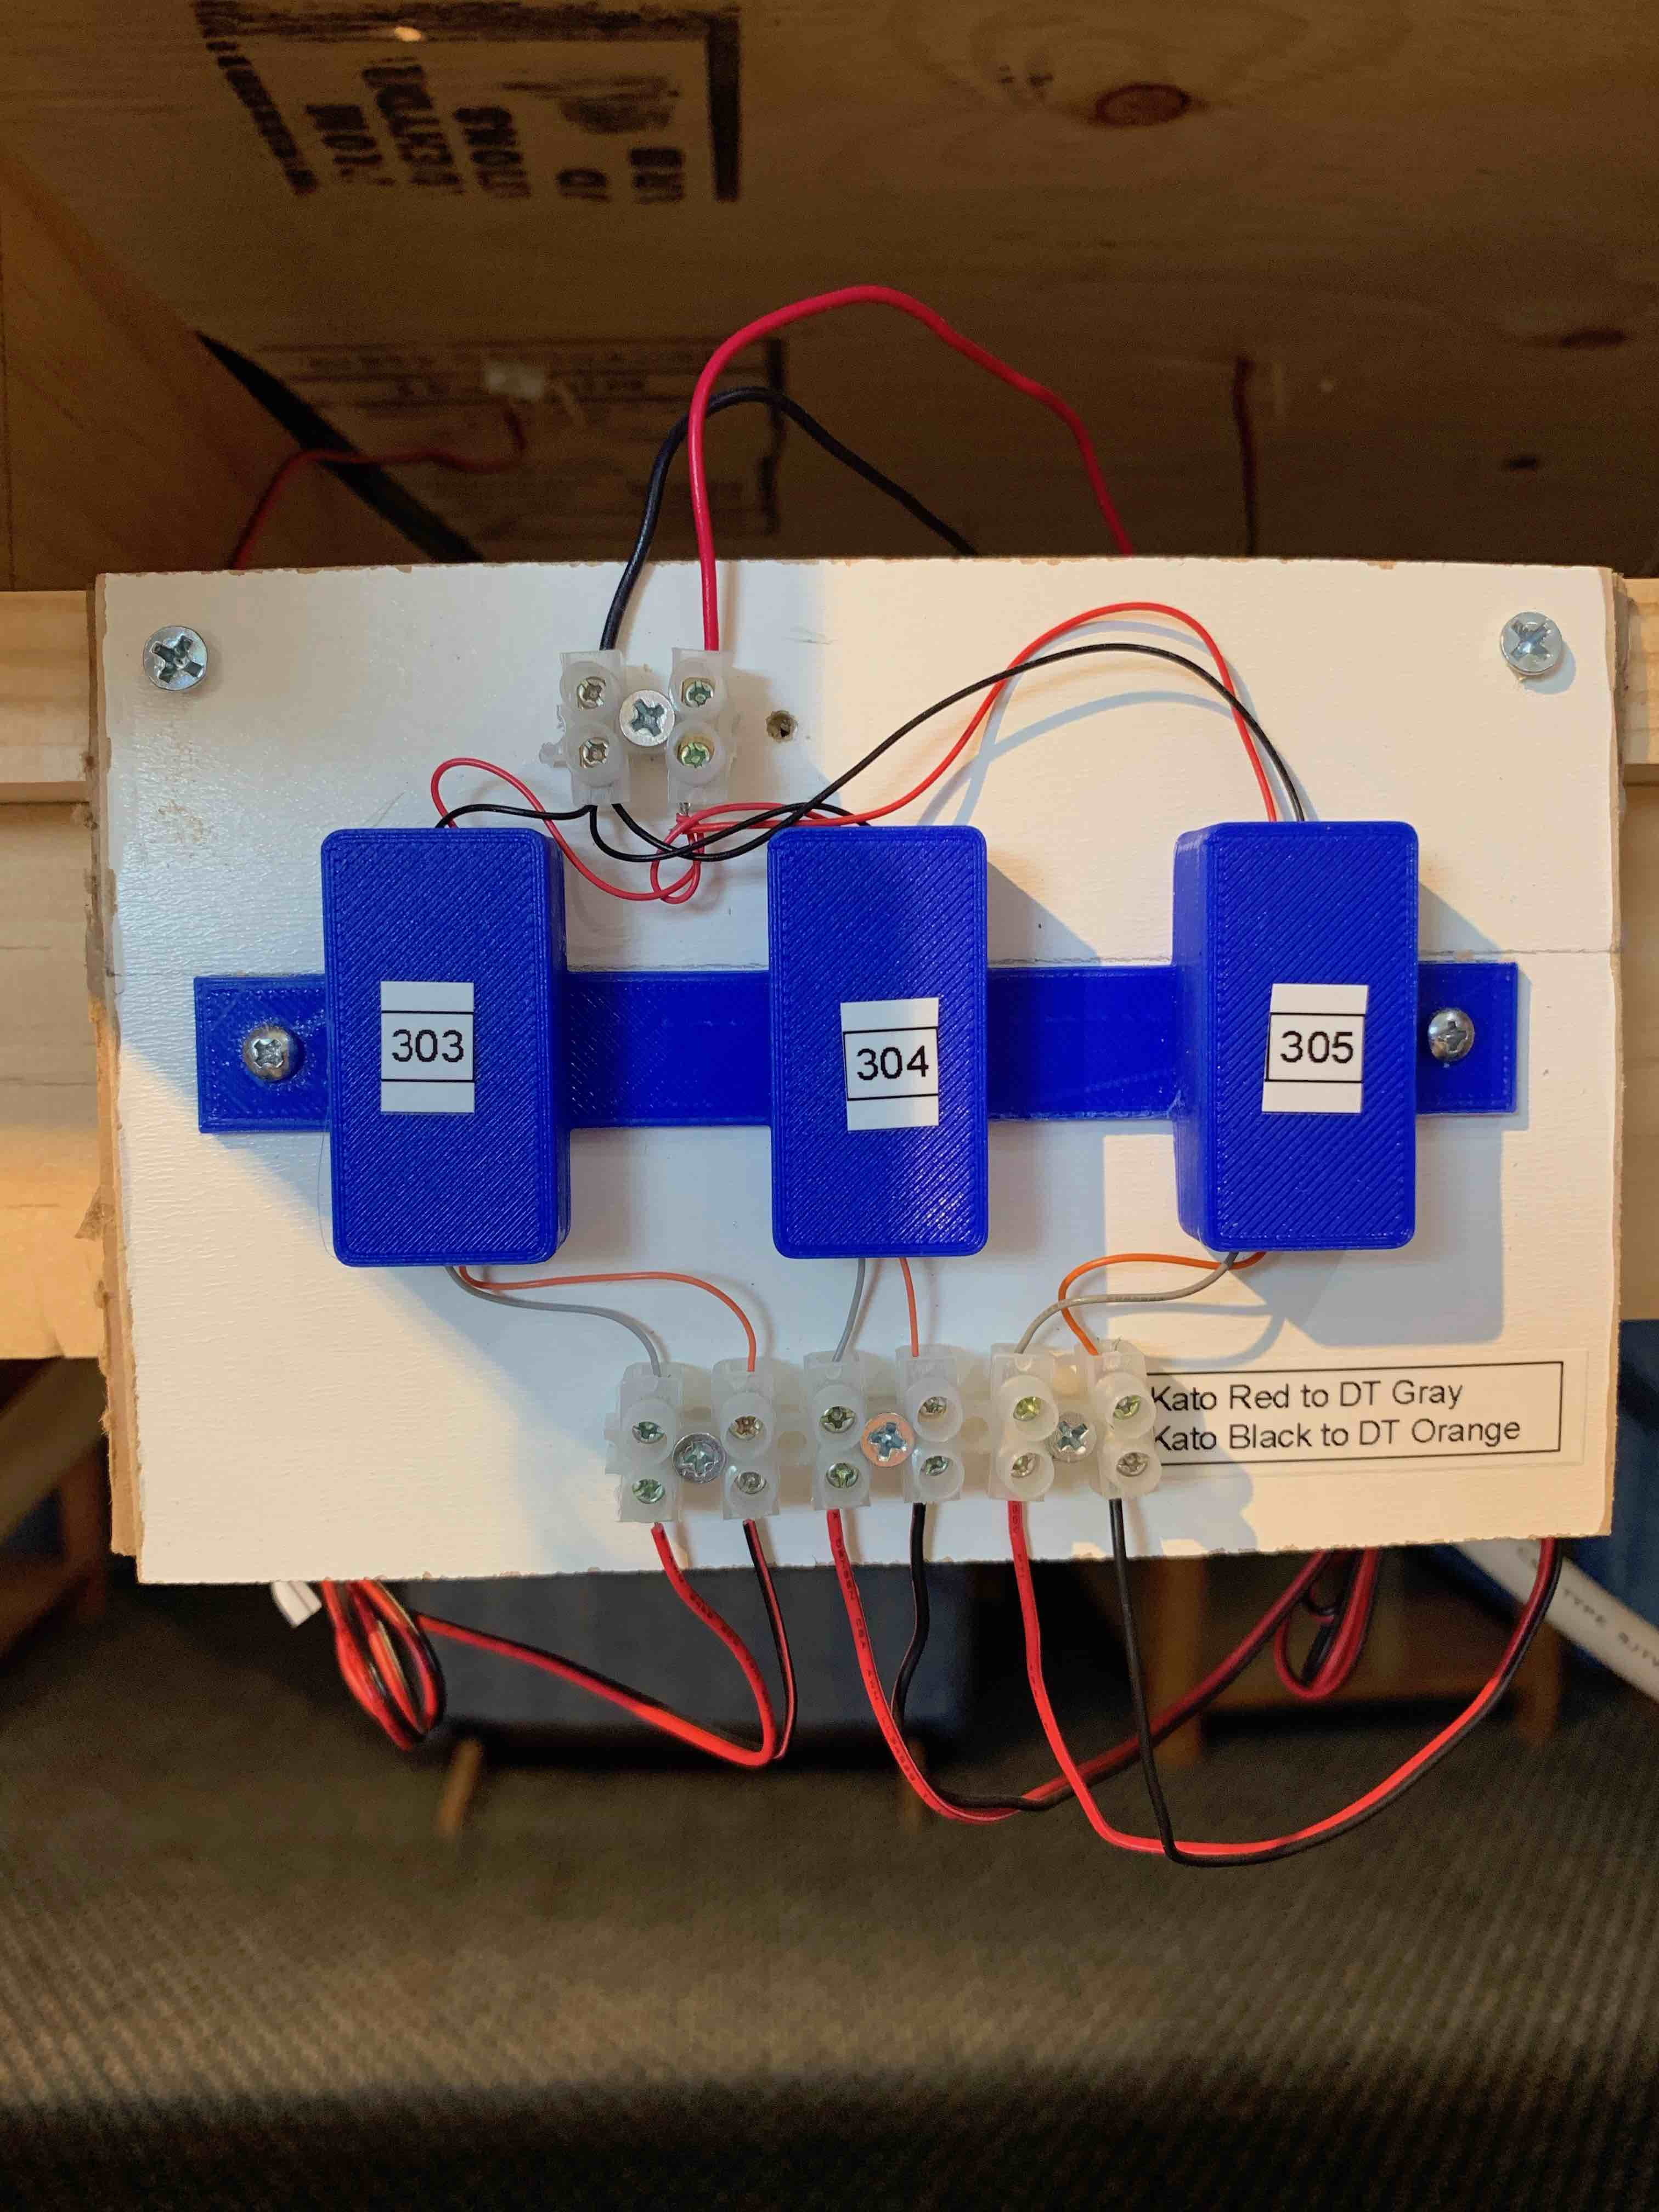
\includegraphics[width=\textwidth]{./3d_printing/figures/ThreeBoxes.jpg}
           \caption{Print of three boxes}
        \end{subfigure}
        \vskip\baselineskip
        \begin{subfigure}[b] {0.475\textwidth}
            \centering 
            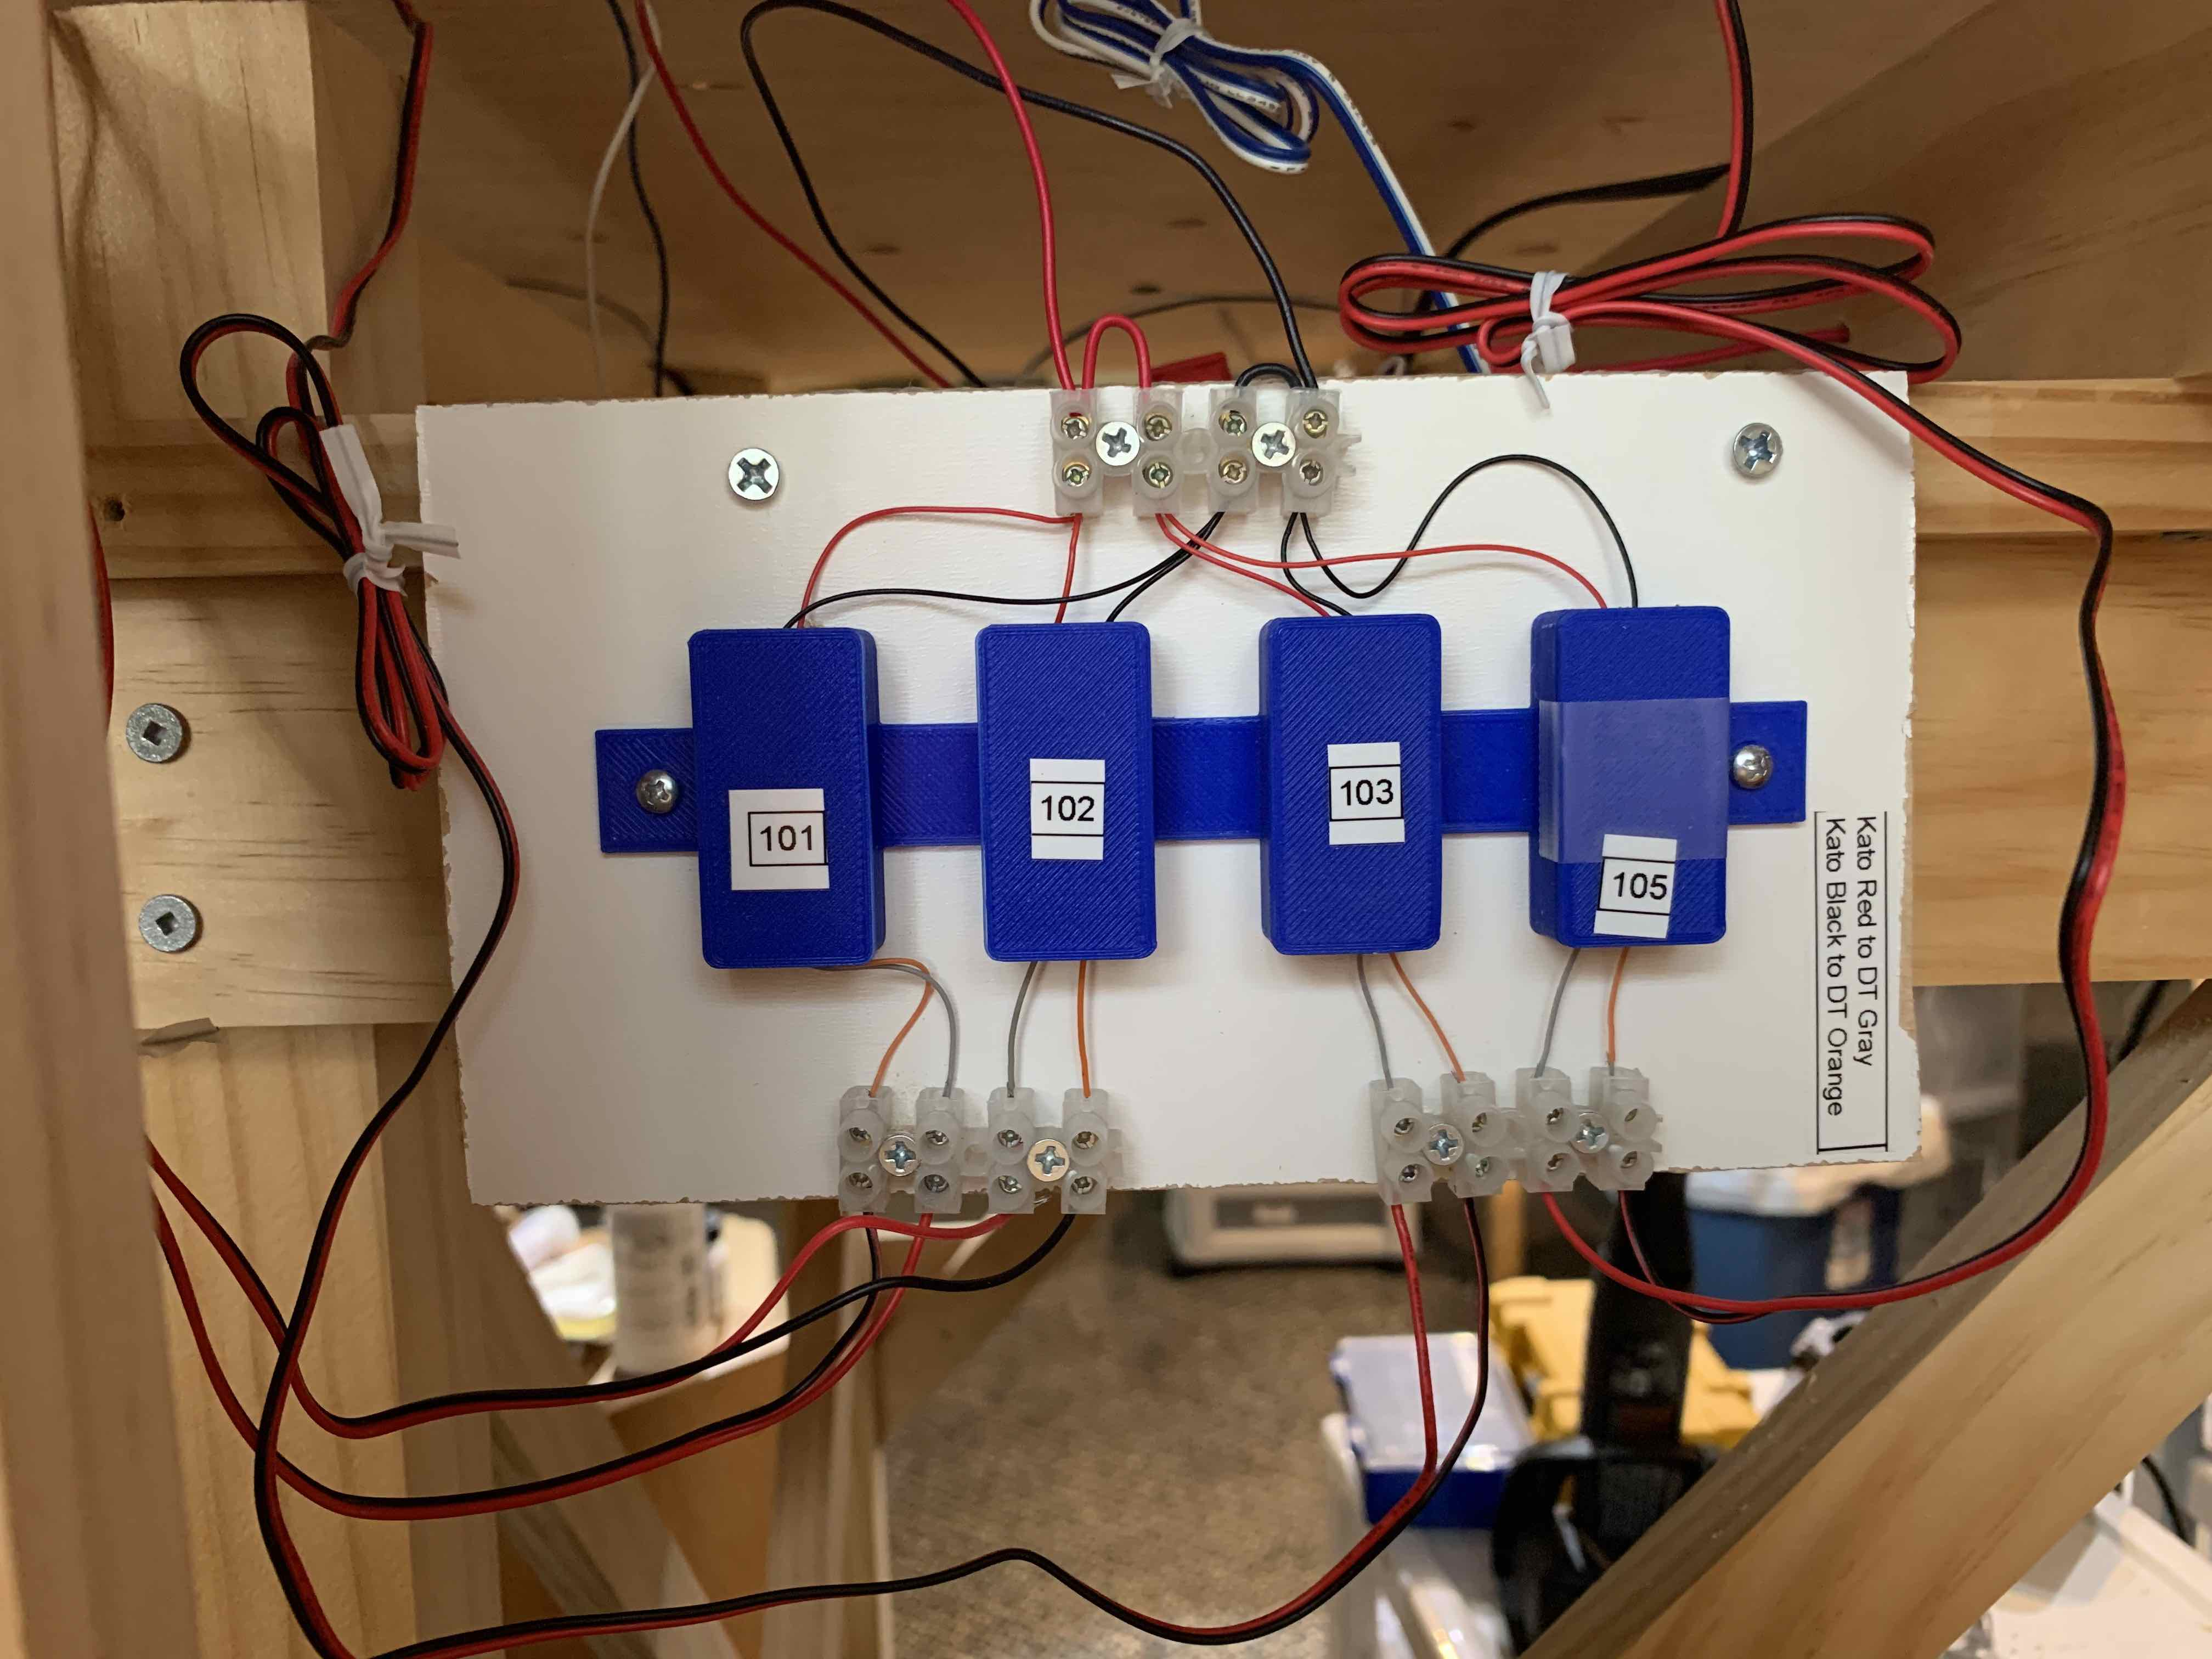
\includegraphics[width=\textwidth]{./3d_printing/figures/FourBoxes.jpg}
         \caption{Print of four boxes}
        \end{subfigure}
        \quad
        \begin{subfigure}[b]  {0.475\textwidth}
            \centering 
            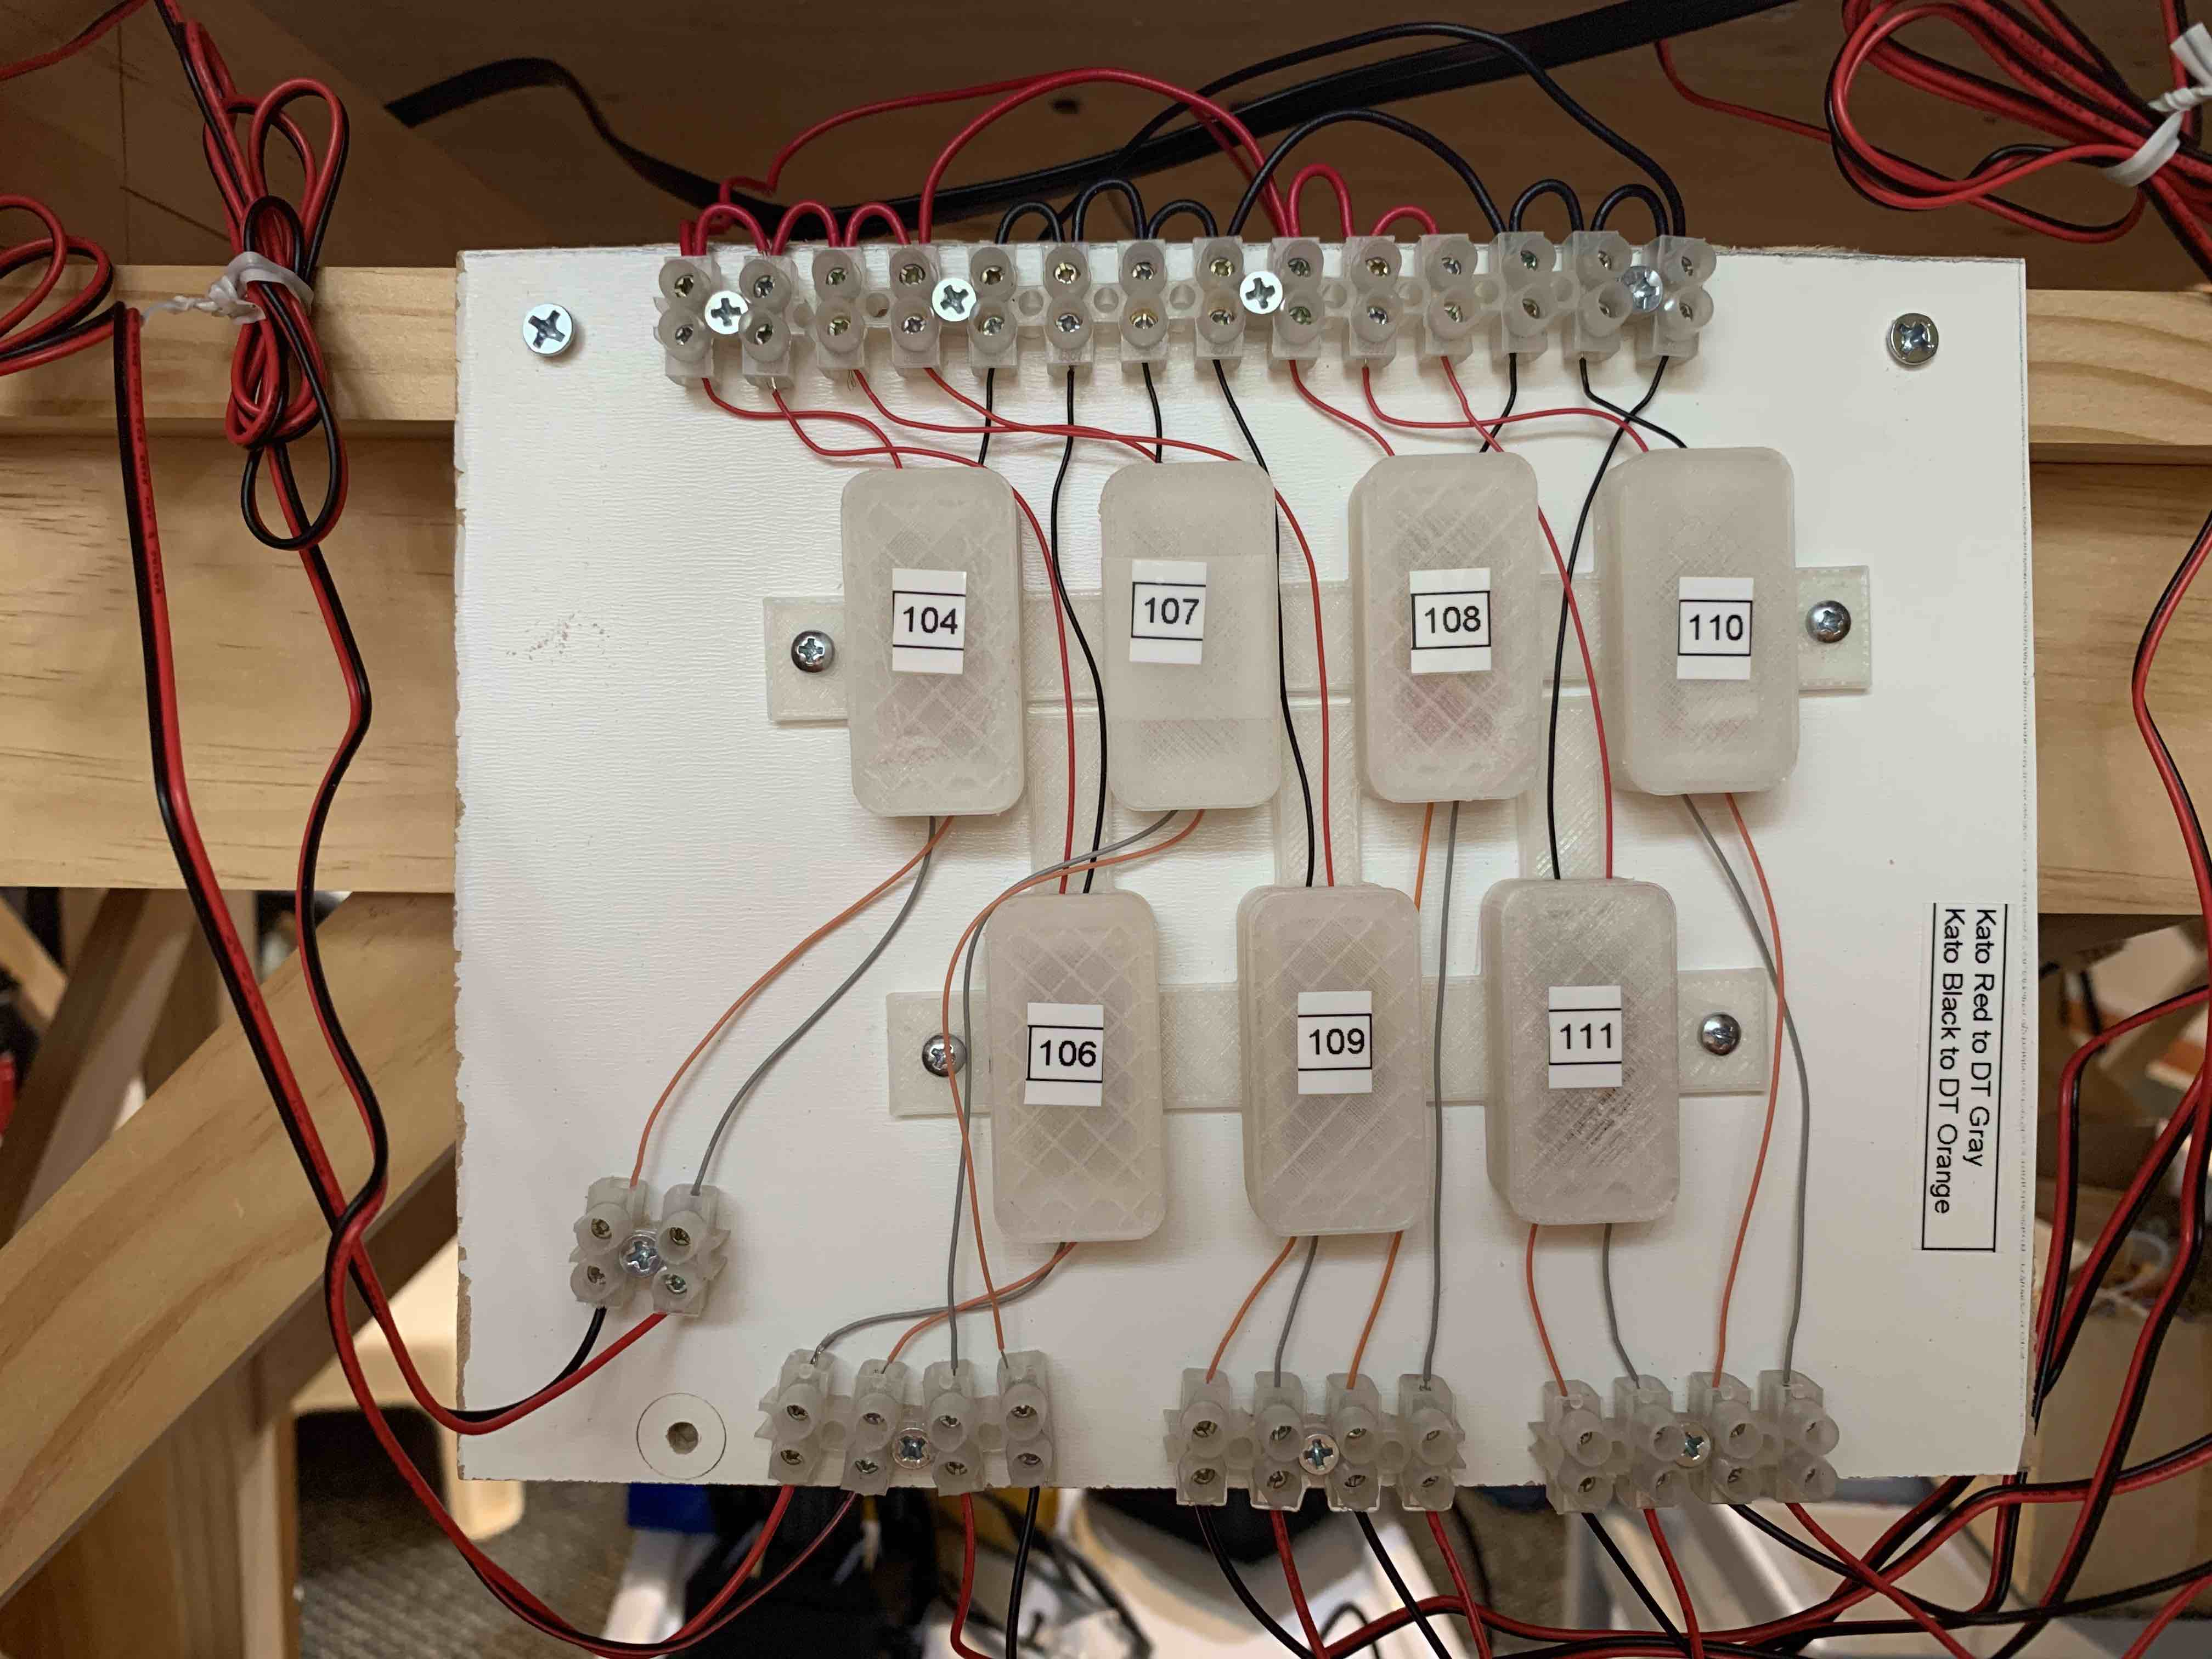
\includegraphics[width=\textwidth]{./3d_printing/figures/SevenBoxes.jpg}
          \caption{Print of seven boxes}
        \end{subfigure}
        \caption {3D assorted size printed boxes to contain accessory decoders for Kato turnouts.} 
        \label{fig:decoderBoxes}
    \end{figure}
    
\section{Printing Structures and Rolling Stock}
To be written.





%%%% Back matter of the book
\backmatter
\refstepcounter{chapter}
\addcontentsline{toc}{chapter}{Index}
\footnotesize
\printindex
\normalsize
\refstepcounter{chapter}

\end{document}
